
\documentclass[fleqn,addpoints]{exam}

\usepackage{graphicx}
\usepackage{booktabs}
\usepackage{float}
\usepackage{amsmath}
\usepackage{cancel}
\usepackage{polynom}
\usepackage{caption}
\usepackage{mdwlist}

\newcommand{\degree}{\ensuremath{^\circ}} 

\printanswers

\ifprintanswers 
\usepackage{2in1, lscape} 
\fi

\title{Math 115 \\ Homework 22}
\date{May 10, 2011}

\begin{document}

\maketitle

% \begin{figure}[H]
%   \centering
%   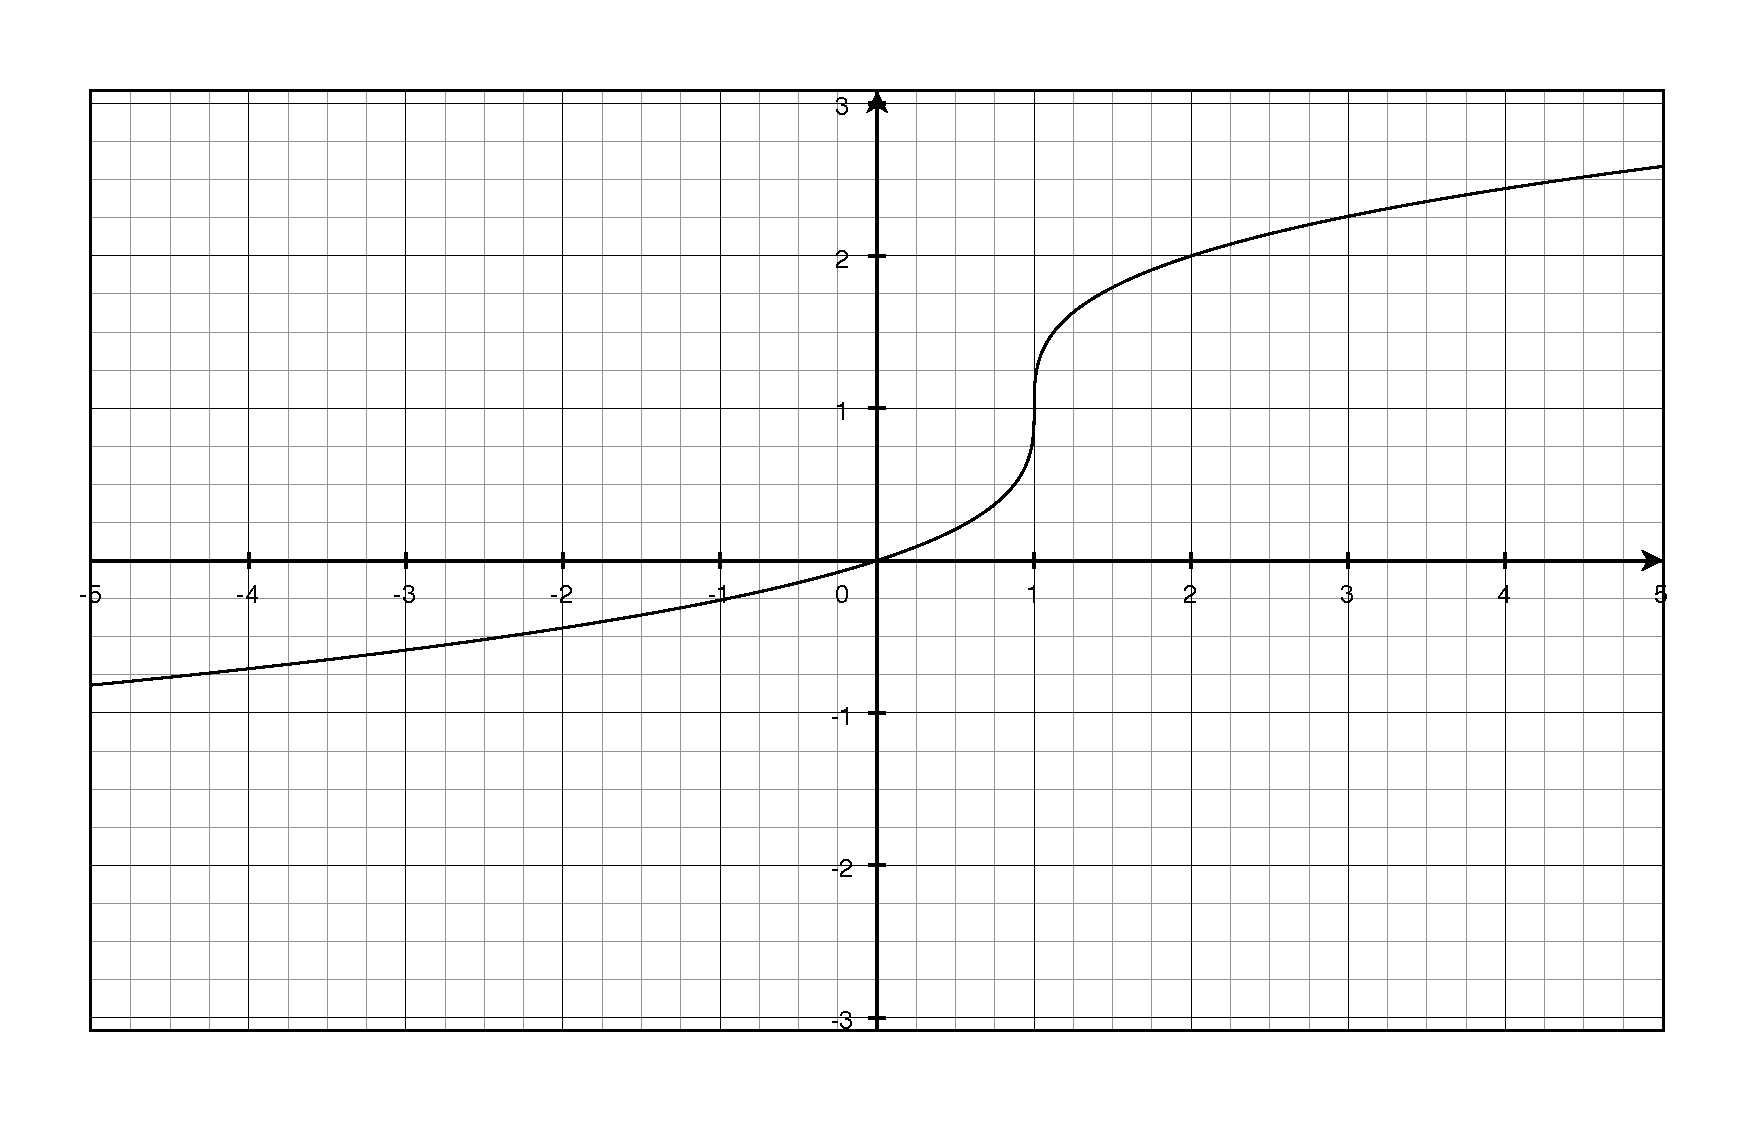
\includegraphics[scale=.3]{question7.eps}
%   \caption*{Question 7}
% \end{figure}

% \begin{tabular}{cc}
% \toprule
% period & amplitude \\
% \midrule
%   $\pi$ & $2$ \\
% \bottomrule
% \end{tabular}

\section{Homework}
\begin{itemize*}
  \item pp 397-400: 1-6, 13-14, 27-28, 31, 33, 35-38, 43-44, 46, 51-52, 61-62, 65-66, 73, 76
  \item pp 408-411: 1-6, 7, 9, 12, 13, 17, 25-28, 73, 75-76 
\end{itemize*}


\section{Extra Credit}
\begin{figure}[H]
  \centering
  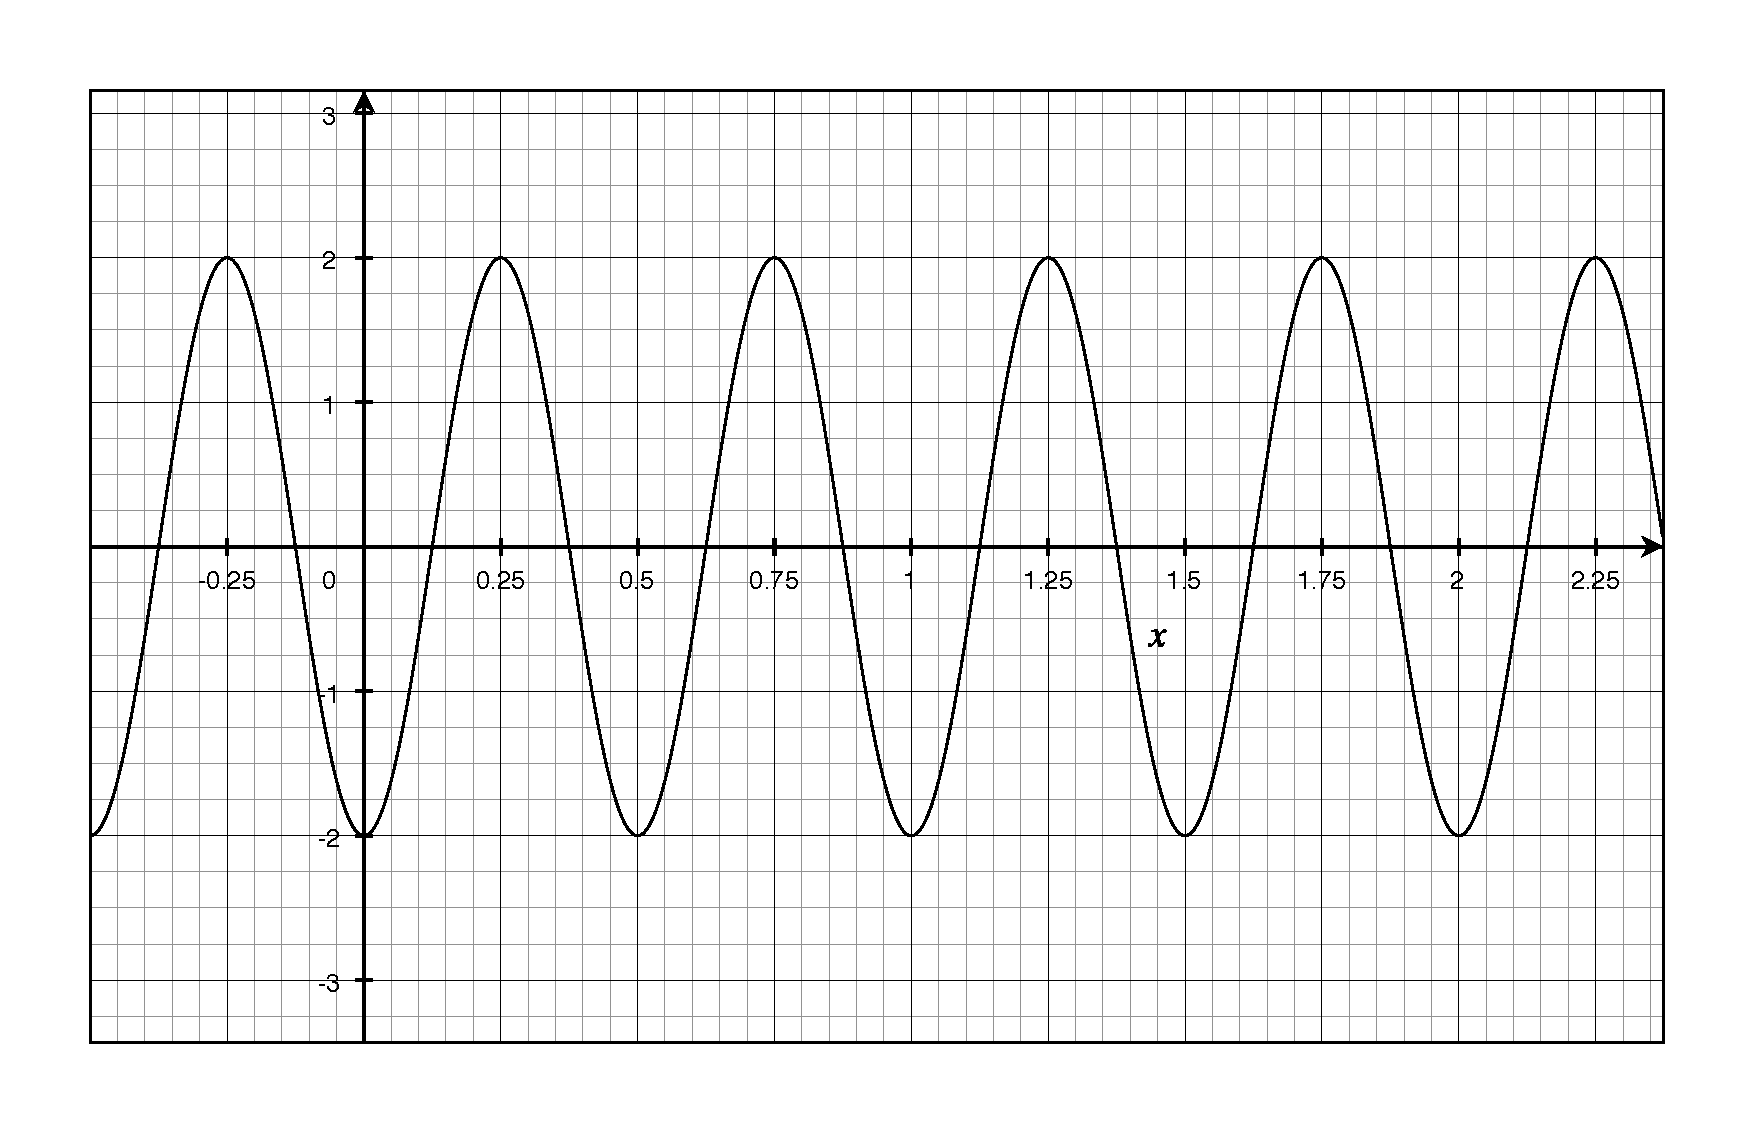
\includegraphics[scale=.4]{extra_credit.eps}
  \caption*{Extra Credit}
\end{figure}

Find 3 different functions which produce this graph.

\begin{solution}

Here are three that work, although these aren't the only three and you may have found different ones.

\begin{align*}
  f(x) = -2 \sin \left( 4 \pi x + \frac{\pi}{2} \right) \\
  g(x) = 2 \sin \left( 4 \pi x - \frac{\pi}{2} \right) \\
  h(x) = -2 \cos(4 \pi x) \\
\end{align*}
\end{solution}


\ifprintanswers
\section{Pages 397-400}

\begin{description}

\item[1] period: $\pi$; amplitude: 3

\item[2] period: $\dfrac{2 \pi}{3}$; amplitude: 2

\item[3] period: $4 \pi$; amplitude: $\dfrac{5}{2}$

\item[4] period: $6 \pi$; amplitude: $3$

\item[5] period: $6$; amplitude: $\dfrac{1}{2}$

\item[6] period: $4$; amplitude: $\dfrac{3}{2}$

\item[13] period: $1$; amplitude: $\dfrac{1}{4}$

\item[14] period: $20$; amplitude: $\dfrac{2}{3}$

\item[27]
\begin{figure}[H]
  \centering
  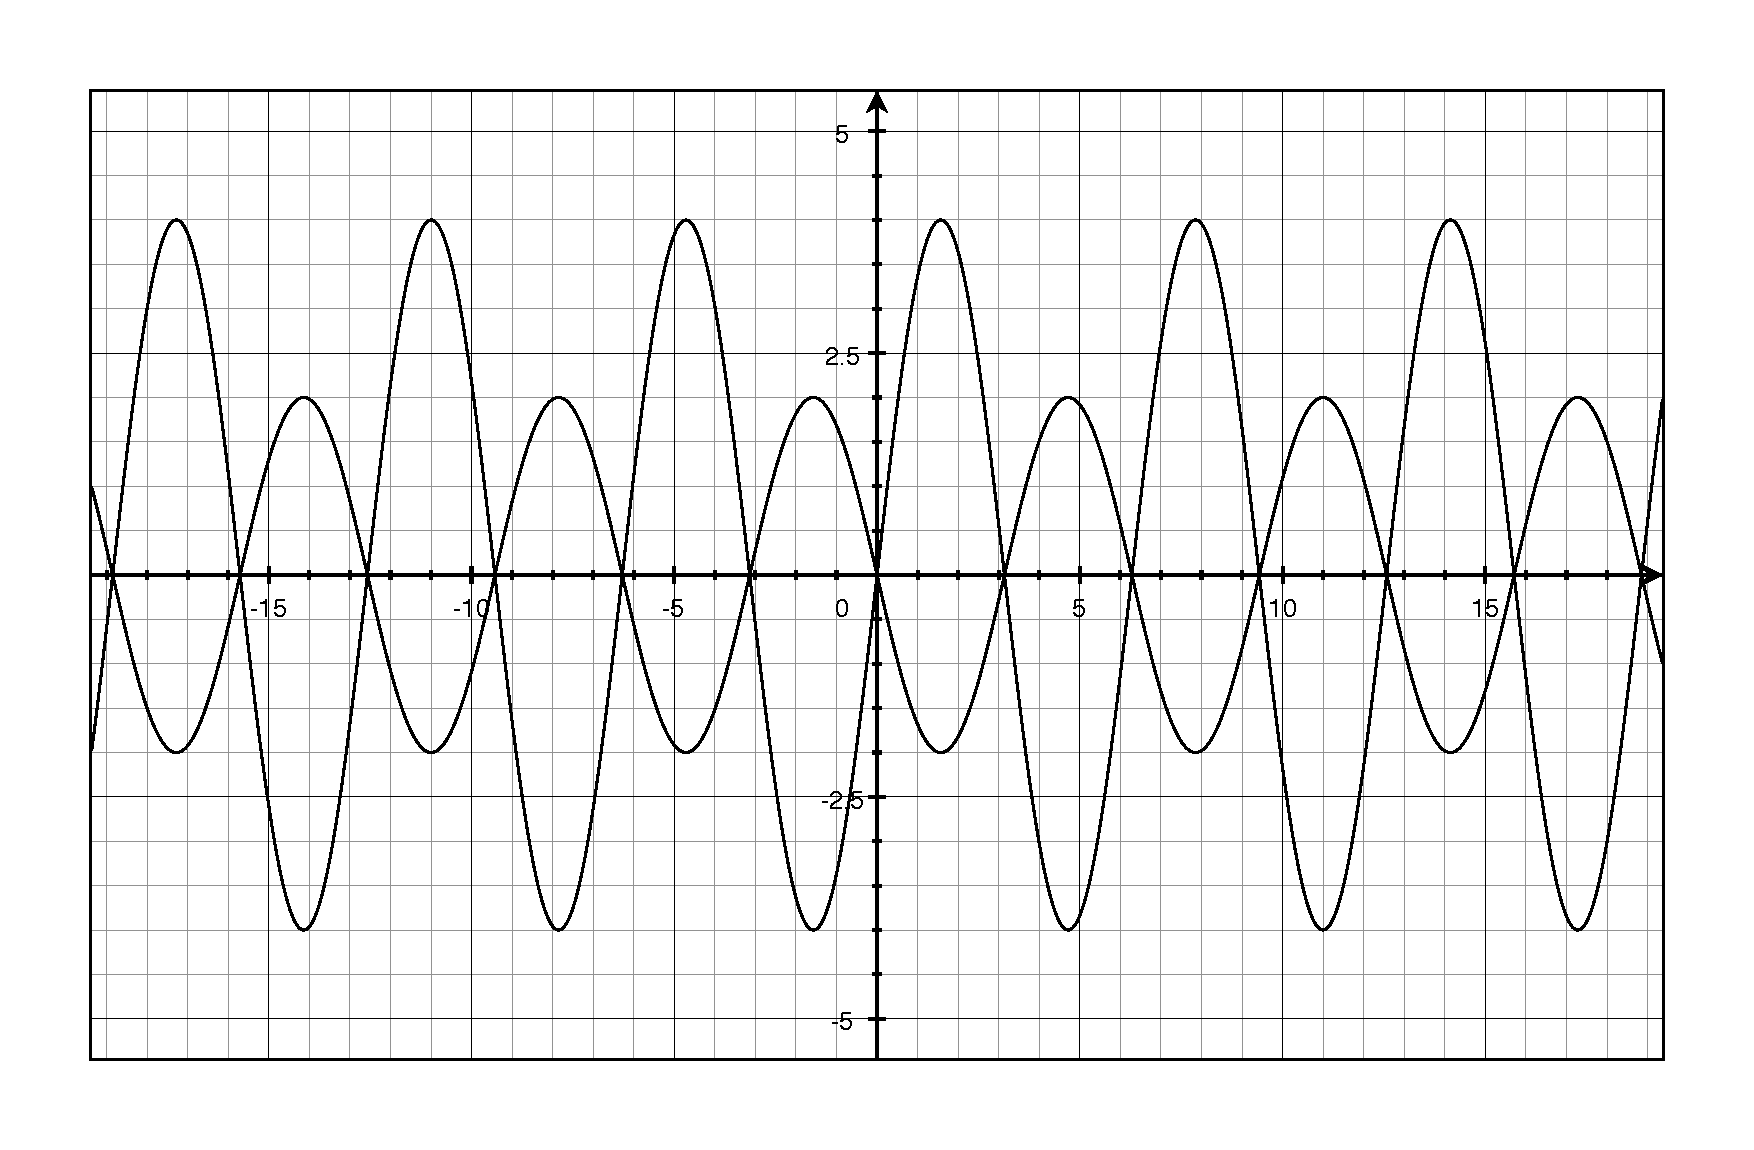
\includegraphics[scale=.3]{question27.eps}
  \caption*{Question 27}
\end{figure}

\item[28]
\begin{figure}[H]
  \centering
  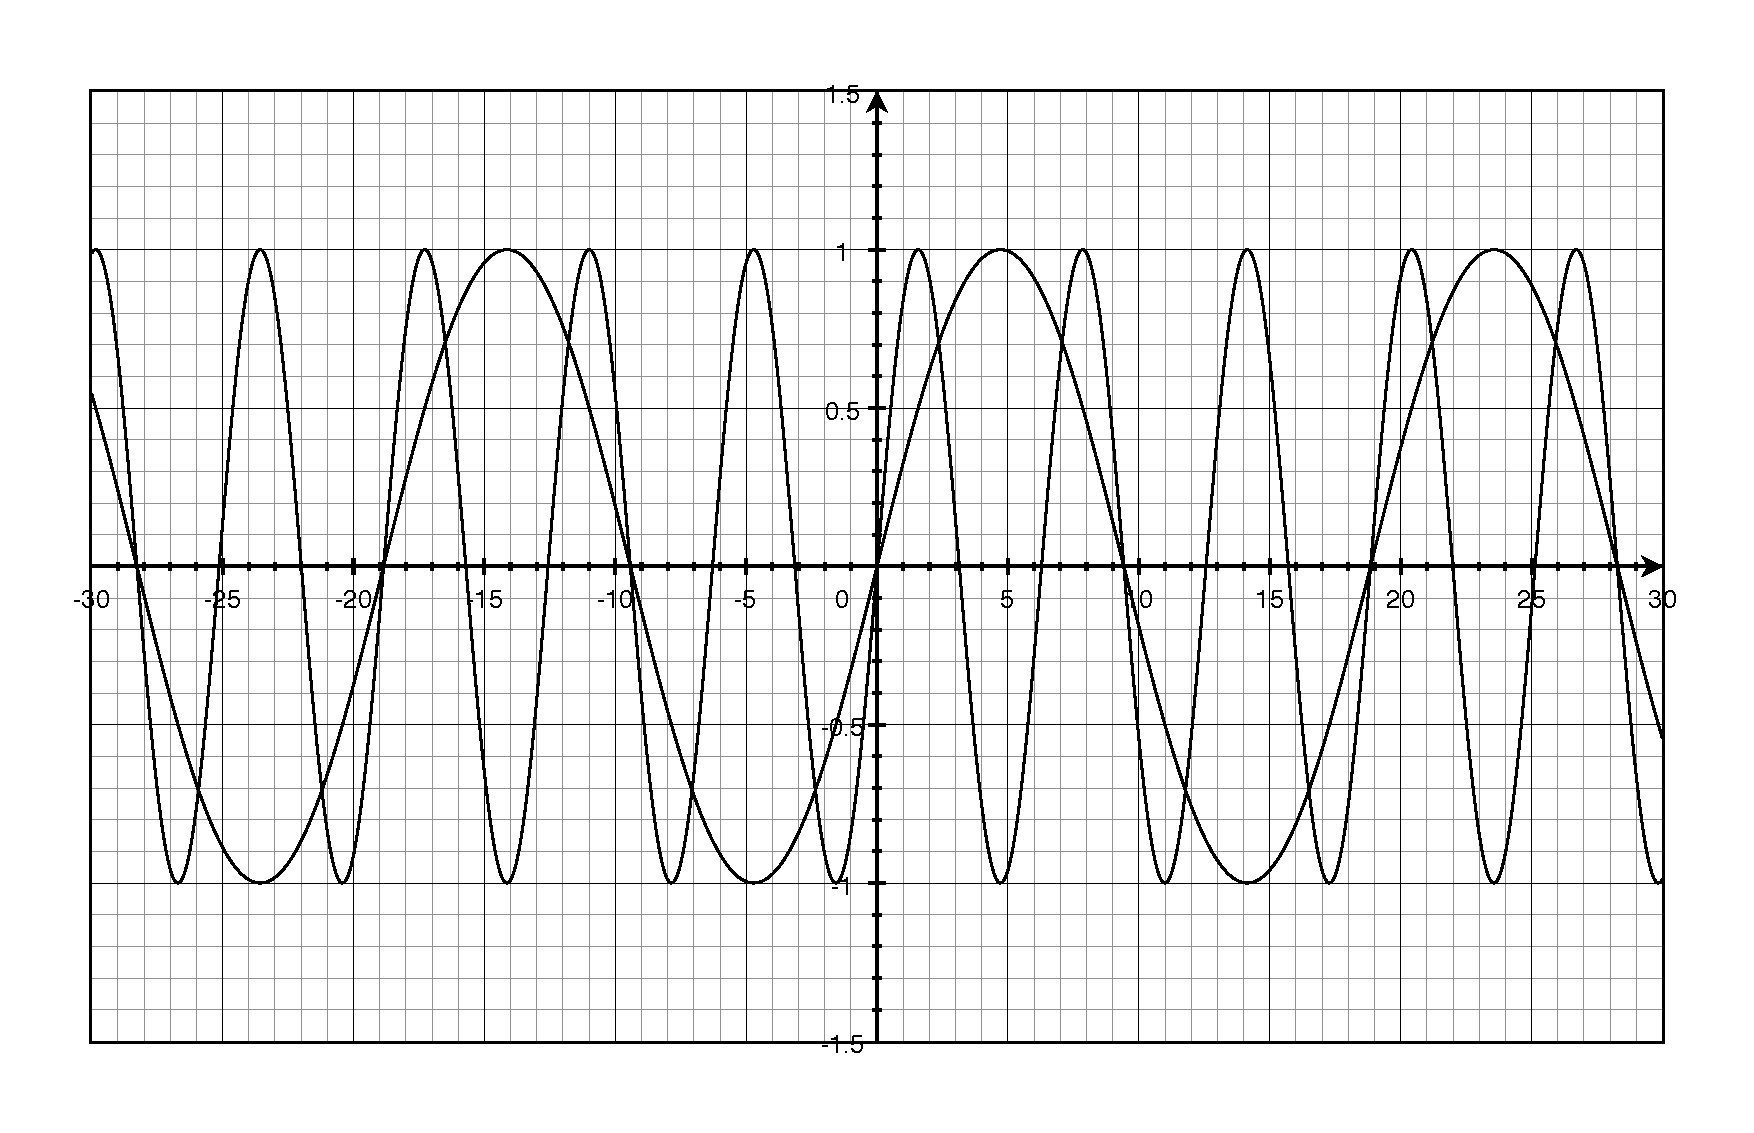
\includegraphics[scale=.3]{question28.eps}
  \caption*{Question 28}
\end{figure}

\item[31]
\begin{figure}[H]
  \centering
  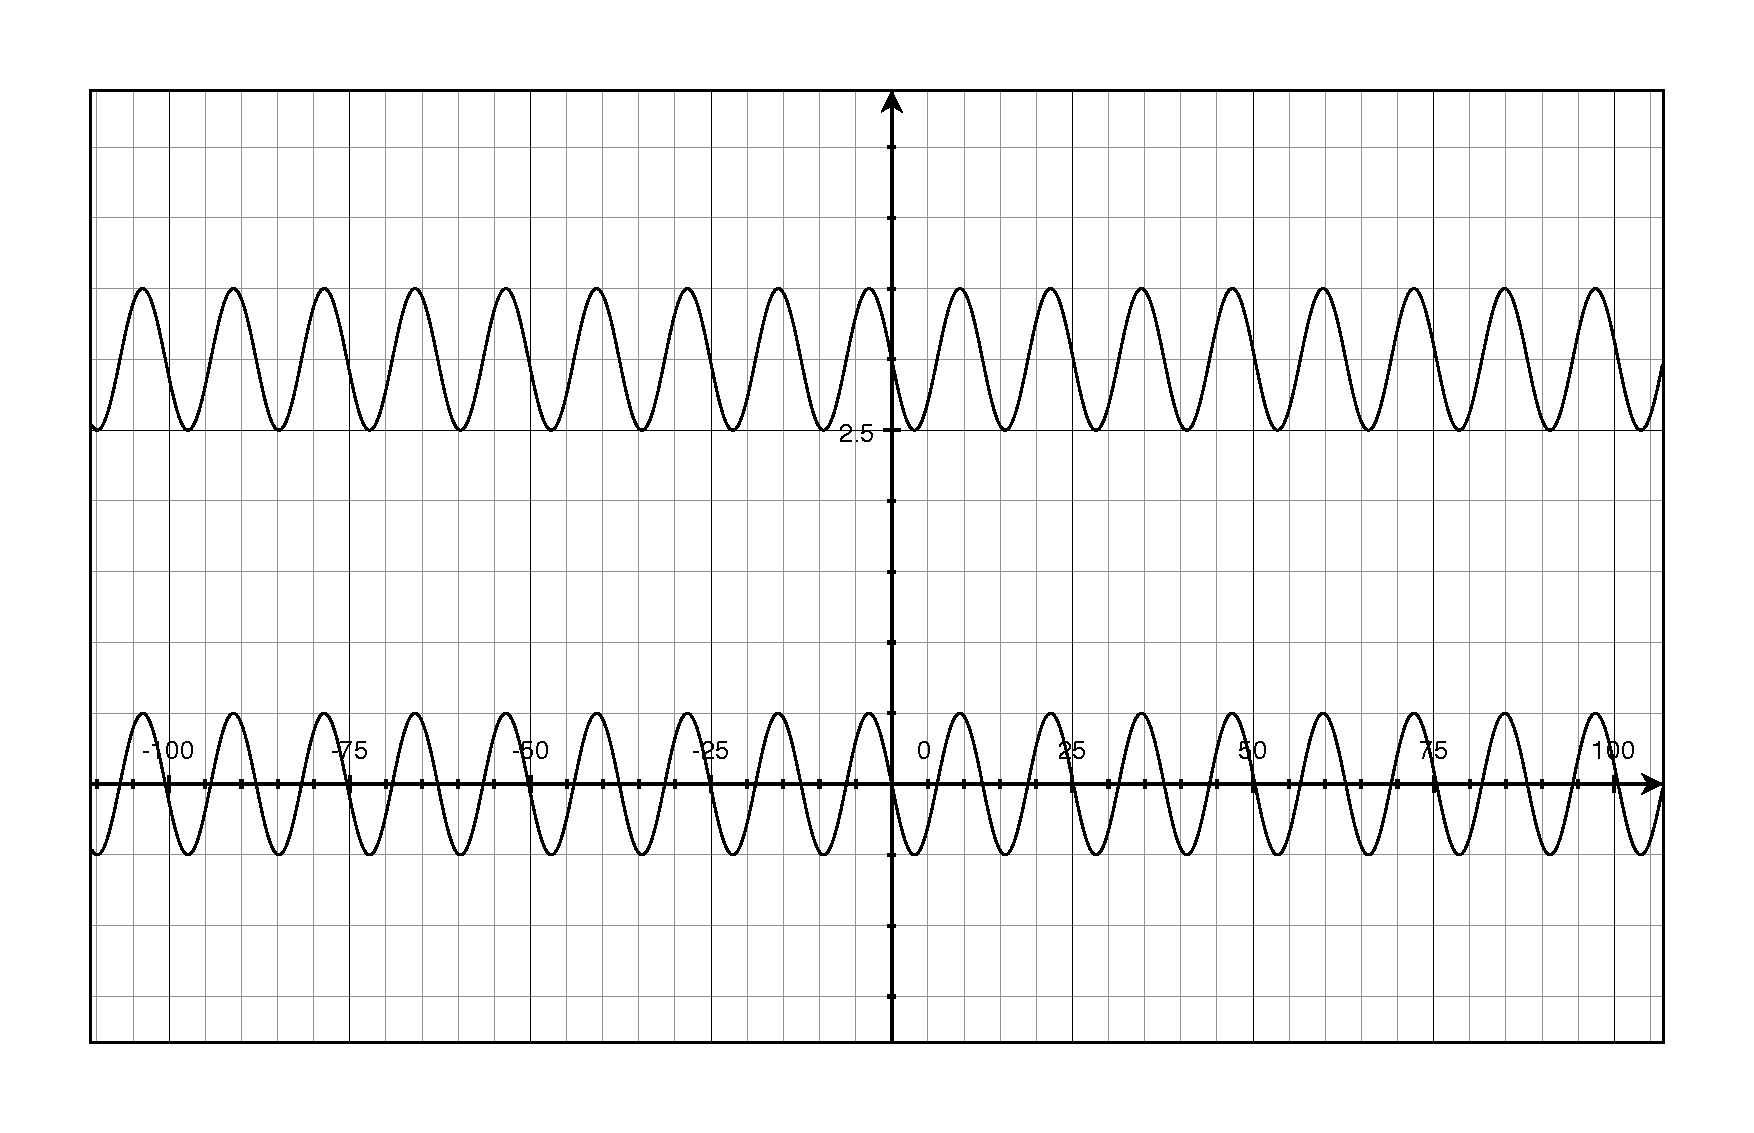
\includegraphics[scale=.3]{question31.eps}
  \caption*{Question 31}
\end{figure}

\item[33]
\begin{figure}[H]
  \centering
  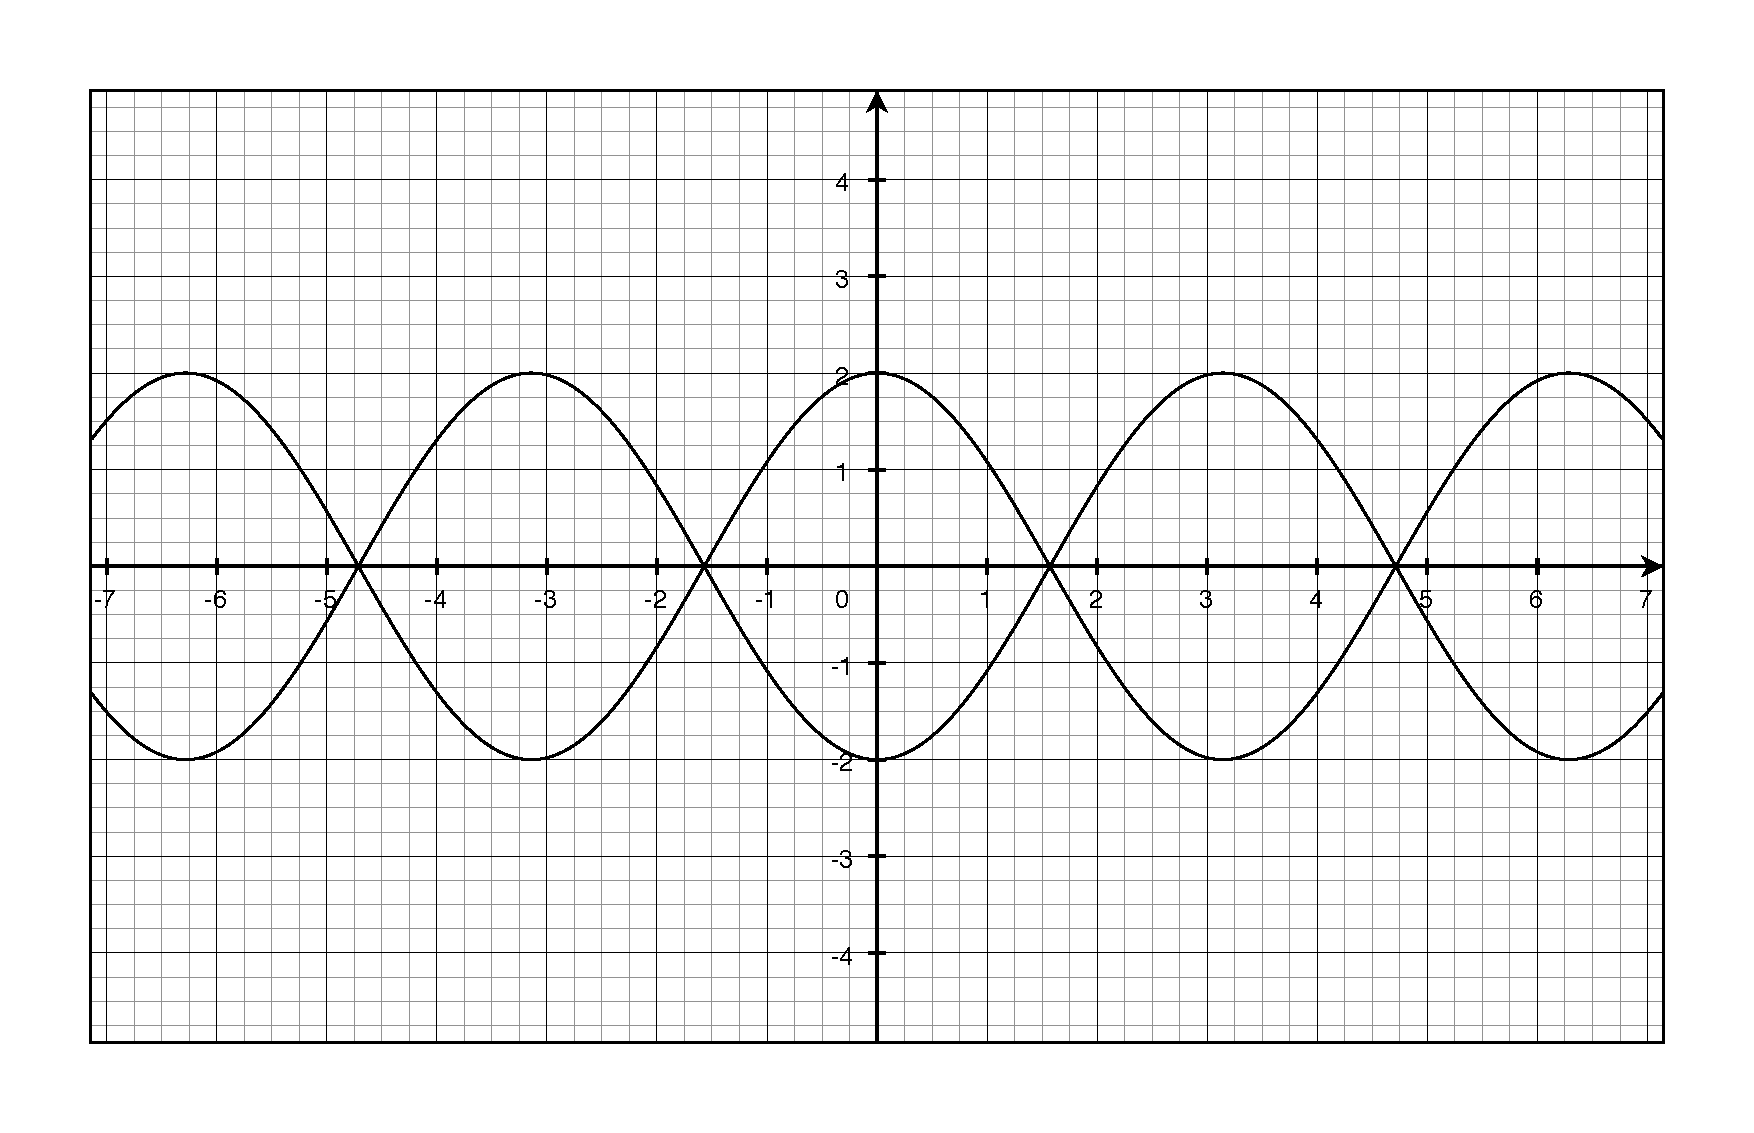
\includegraphics[scale=.3]{question33.eps}
  \caption*{Question 33}
\end{figure}

\item[35]
\begin{figure}[H]
  \centering
  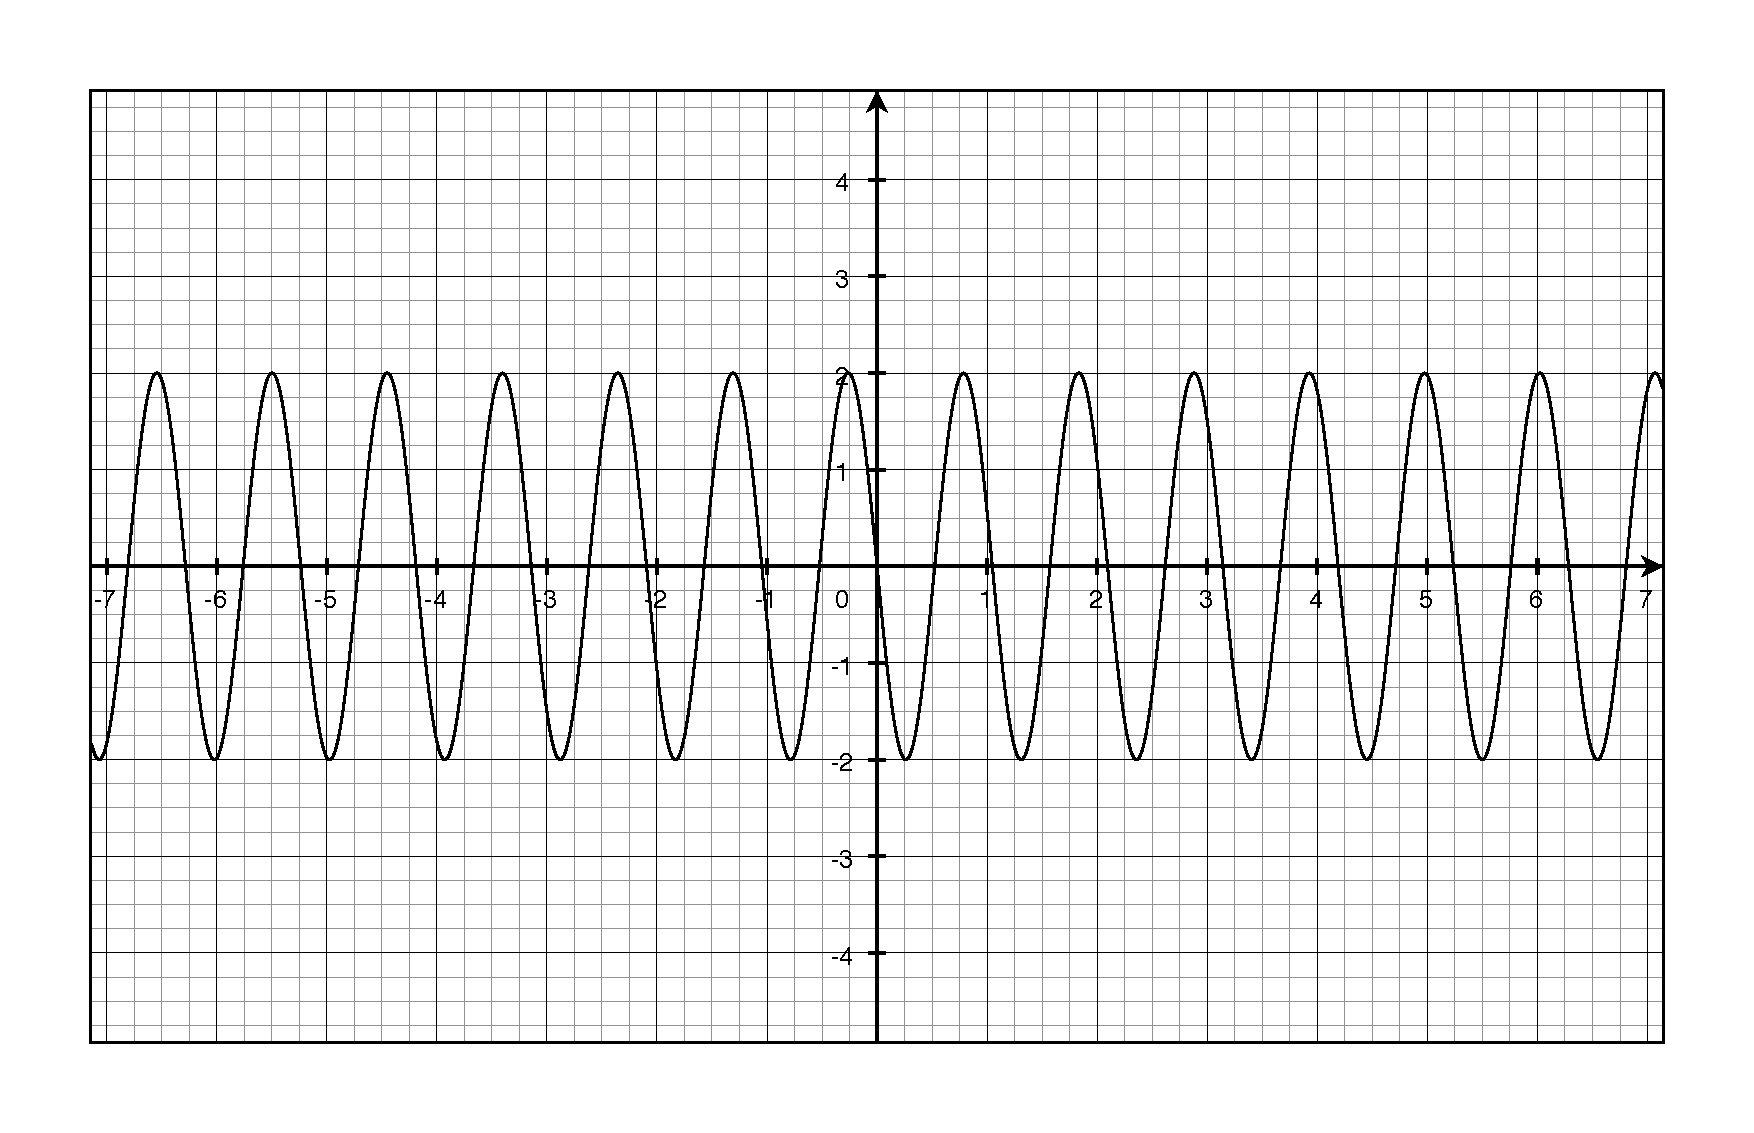
\includegraphics[scale=.3]{question35.eps}
  \caption*{Question 35}
\end{figure}

\item[36]
\begin{figure}[H]
  \centering
  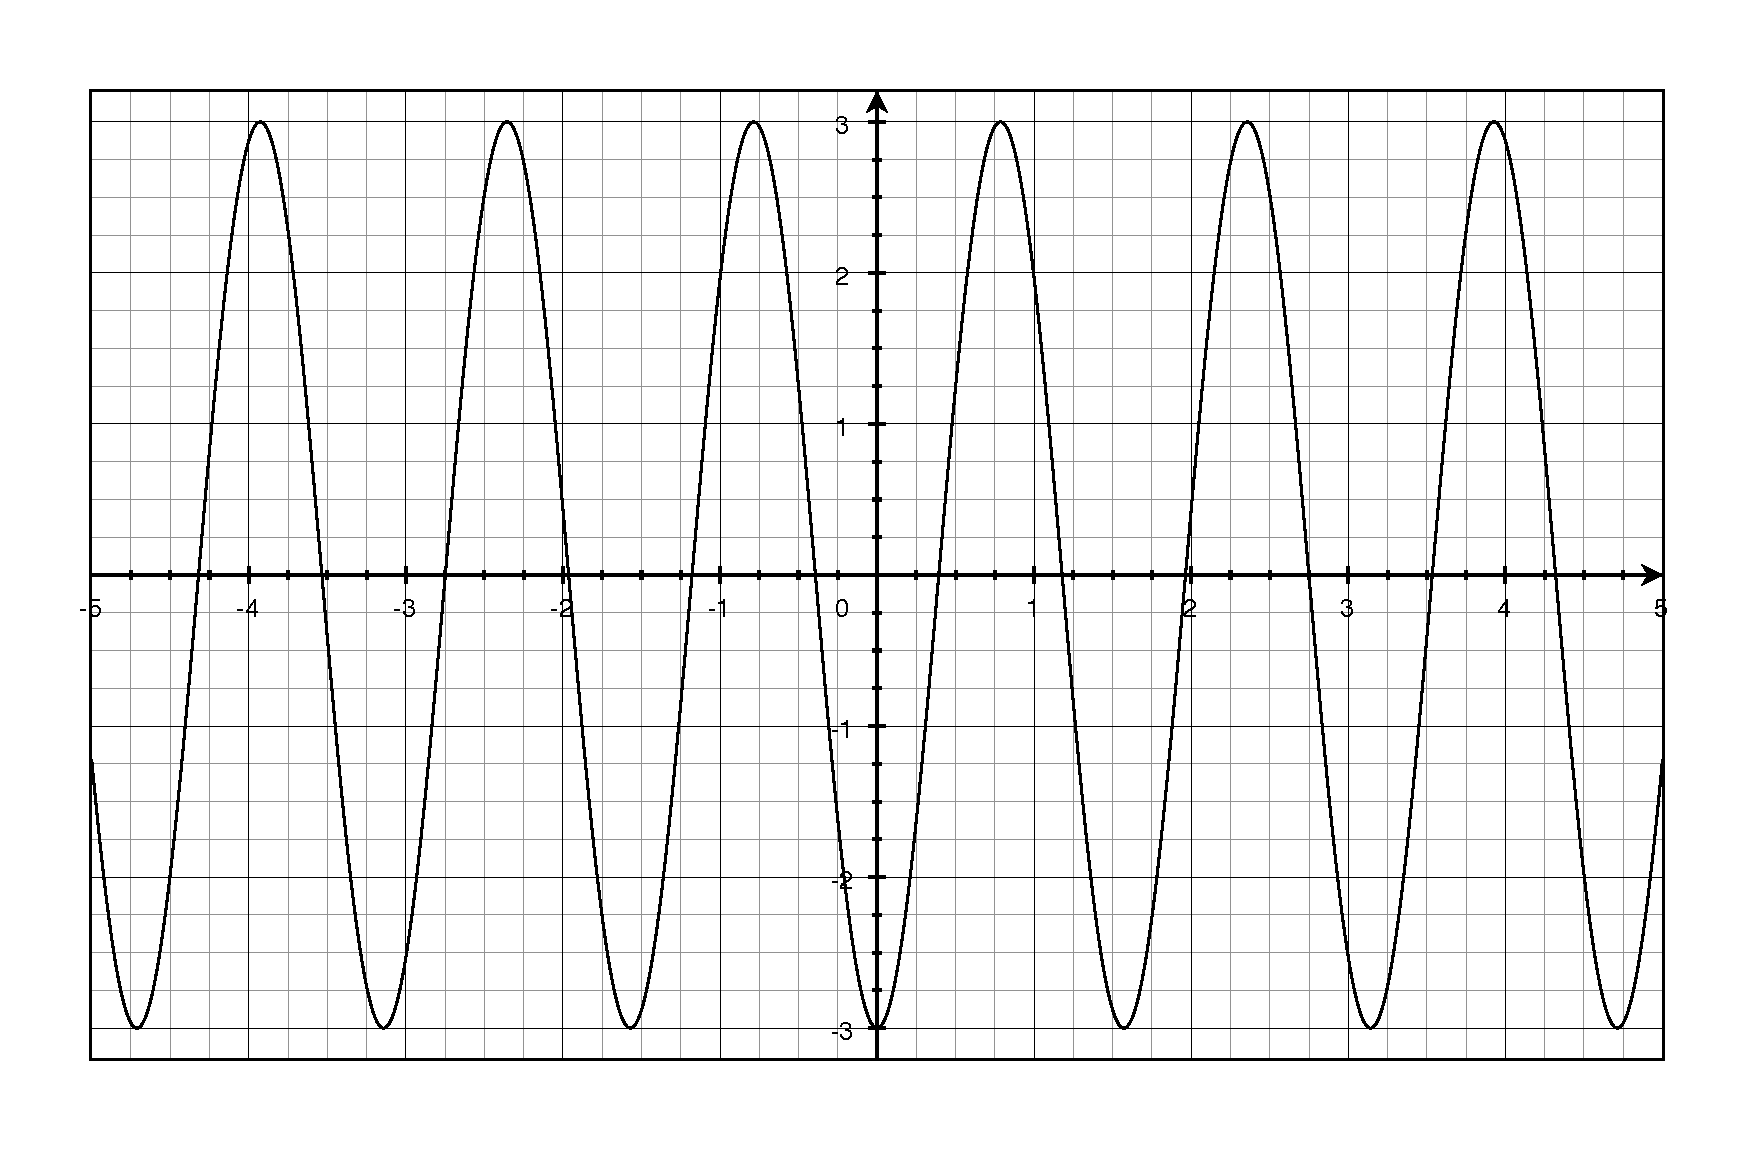
\includegraphics[scale=.3]{question36.eps}
  \caption*{Question 36}
\end{figure}

\item[37]
\begin{figure}[H]
  \centering
  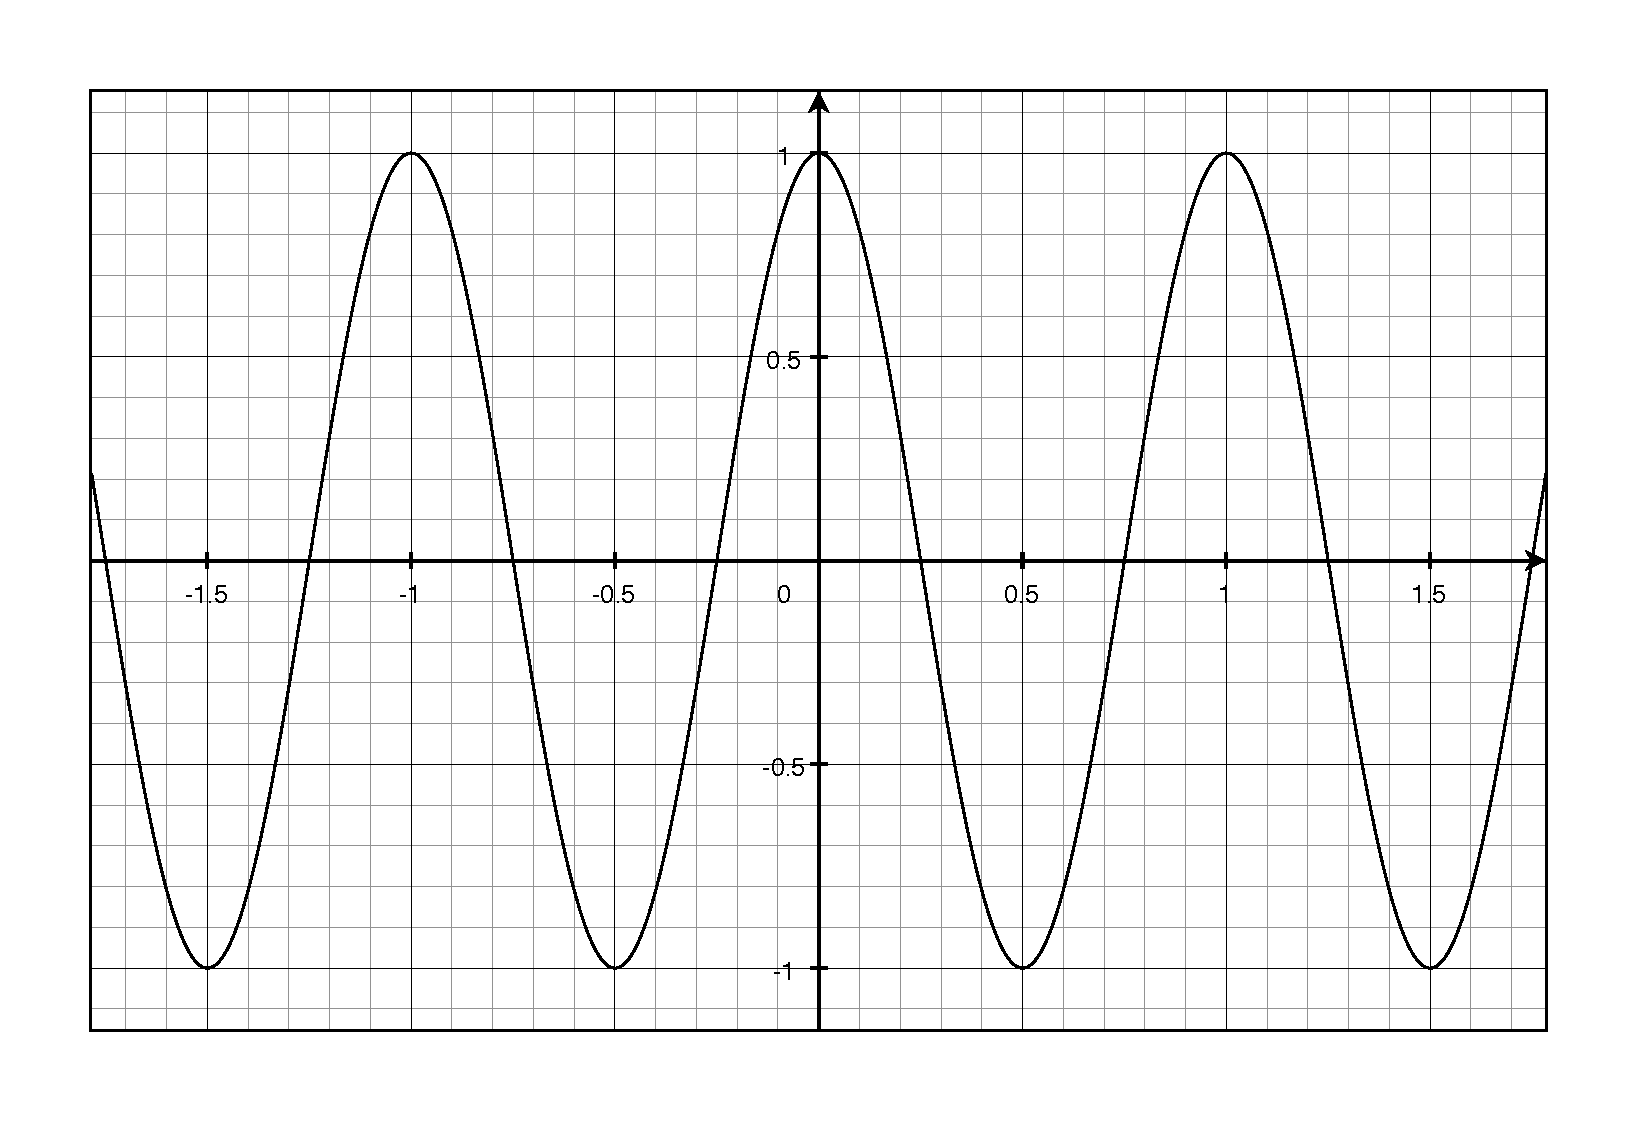
\includegraphics[scale=.3]{question37.eps}
  \caption*{Question 37}
\end{figure}

\item[38]
\begin{figure}[H]
  \centering
  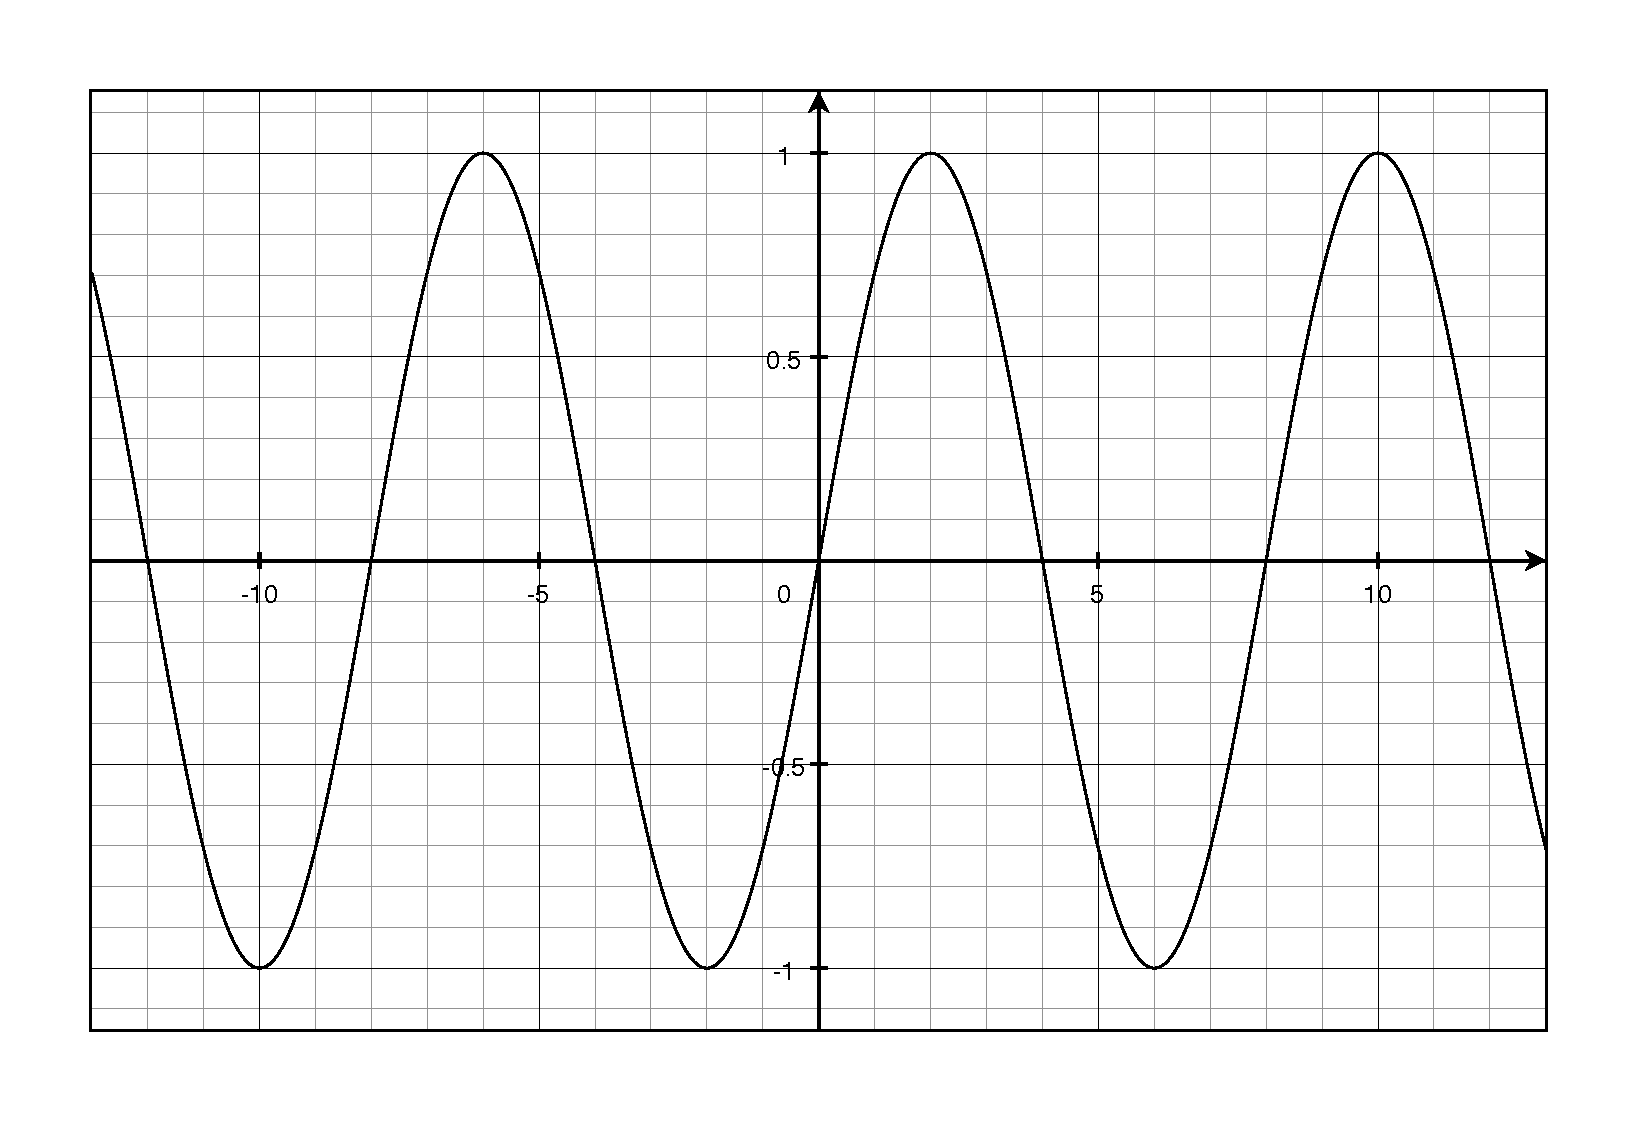
\includegraphics[scale=.3]{question38.eps}
  \caption*{Question 38}
\end{figure}

\item[43]
\begin{figure}[H]
  \centering
  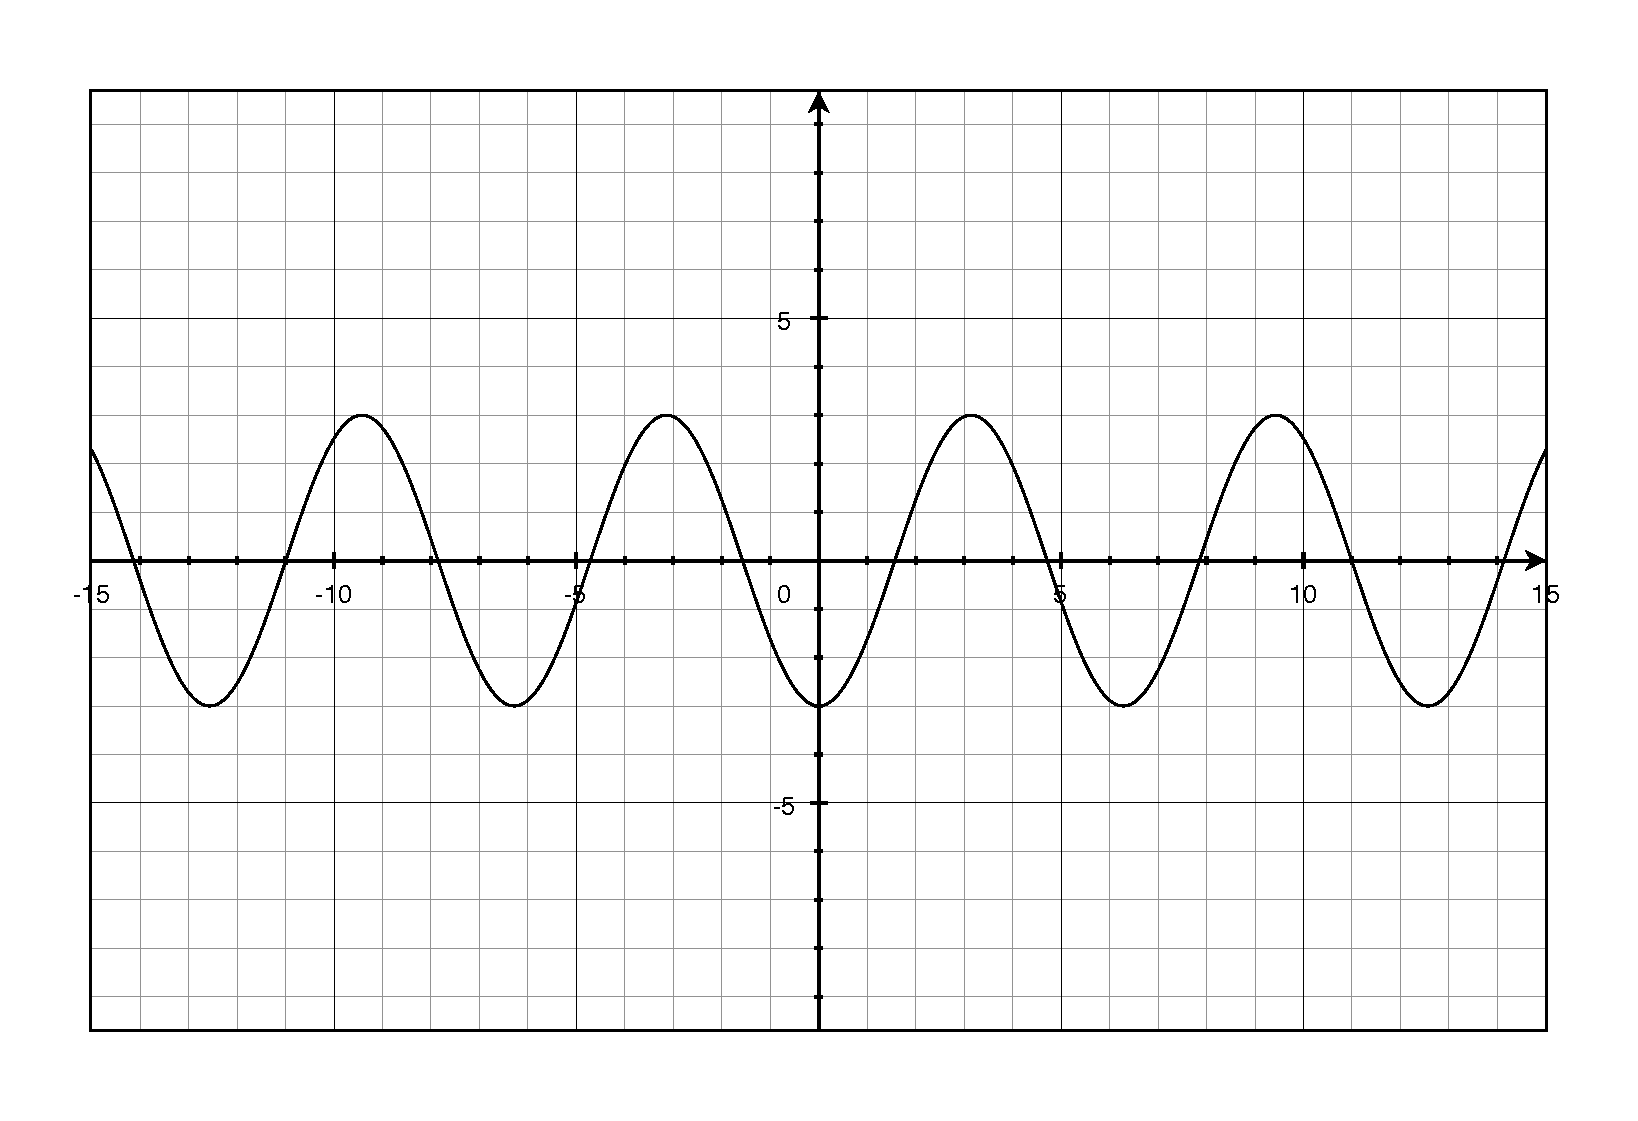
\includegraphics[scale=.3]{question43.eps}
  \caption*{Question 43}
\end{figure}

\item[44]
\begin{figure}[H]
  \centering
  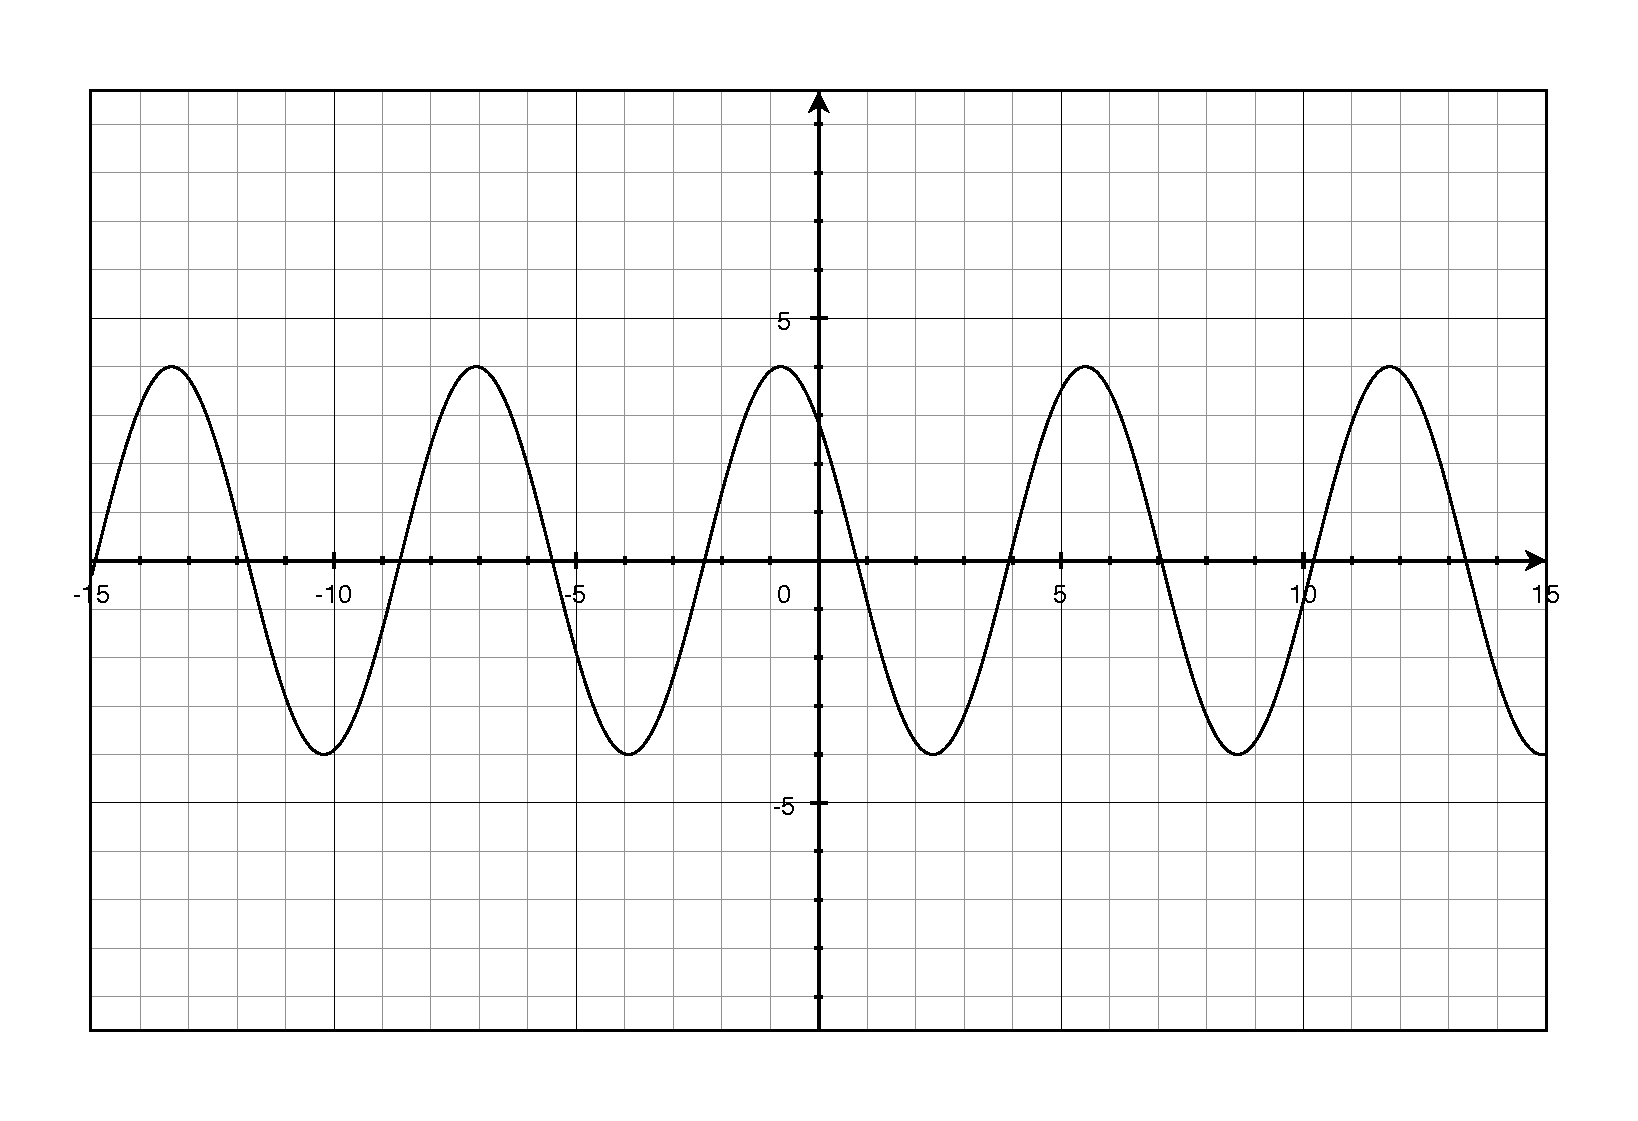
\includegraphics[scale=.3]{question44.eps}
  \caption*{Question 44}
\end{figure}

\item[46]
\begin{figure}[H]
  \centering
  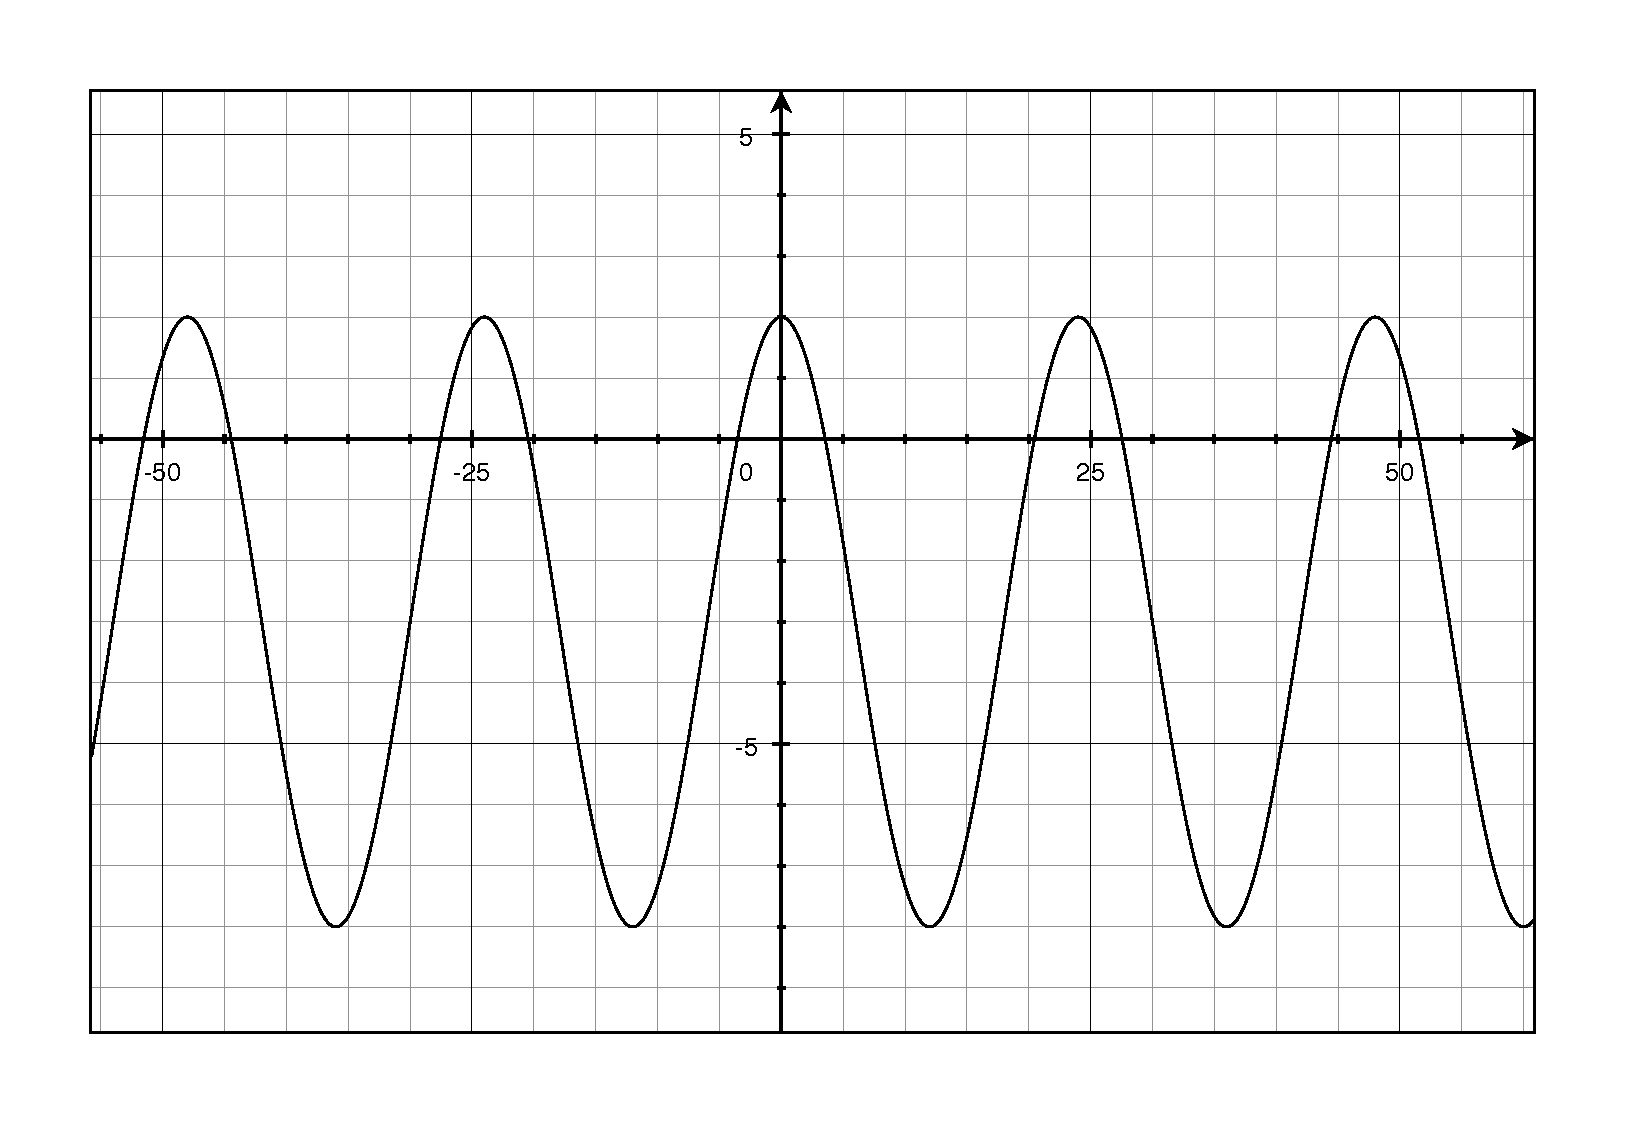
\includegraphics[scale=.3]{question46.eps}
  \caption*{Question 46}
\end{figure}

\item[51]
\begin{figure}[H]
  \centering
  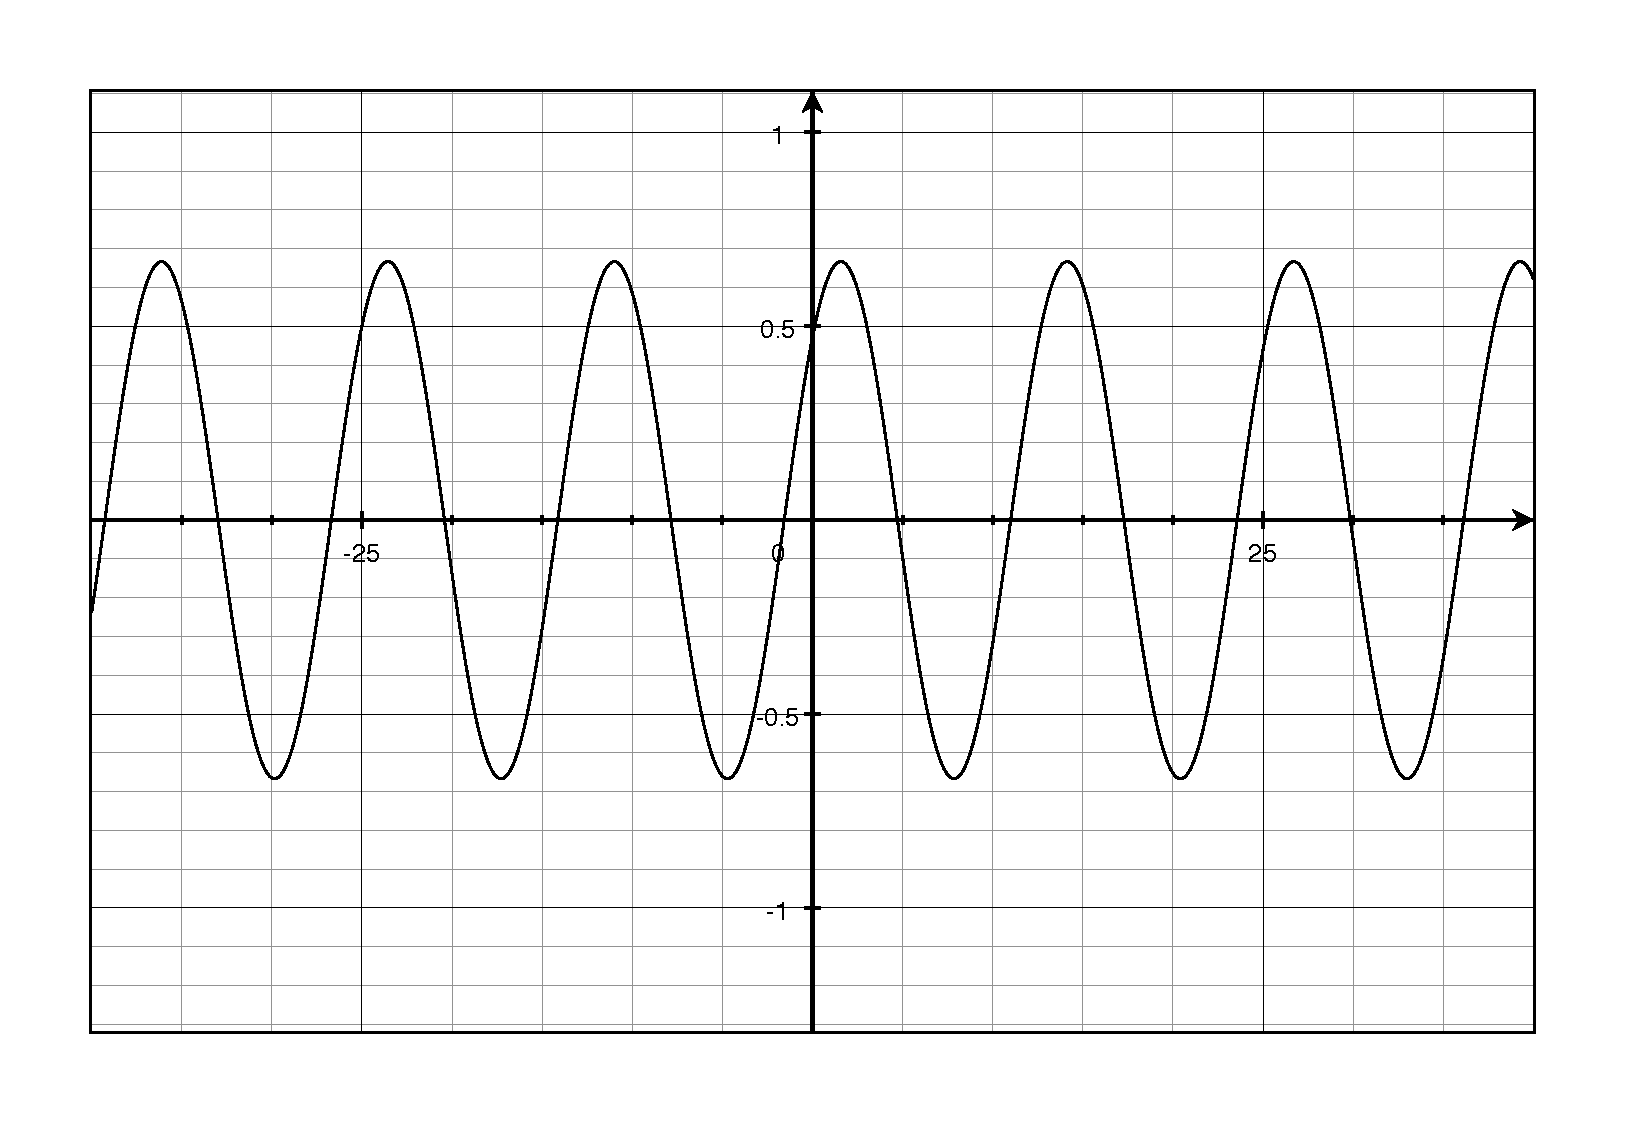
\includegraphics[scale=.3]{question51.eps}
  \caption*{Question 51}
\end{figure}

\item[52]
\begin{figure}[H]
  \centering
  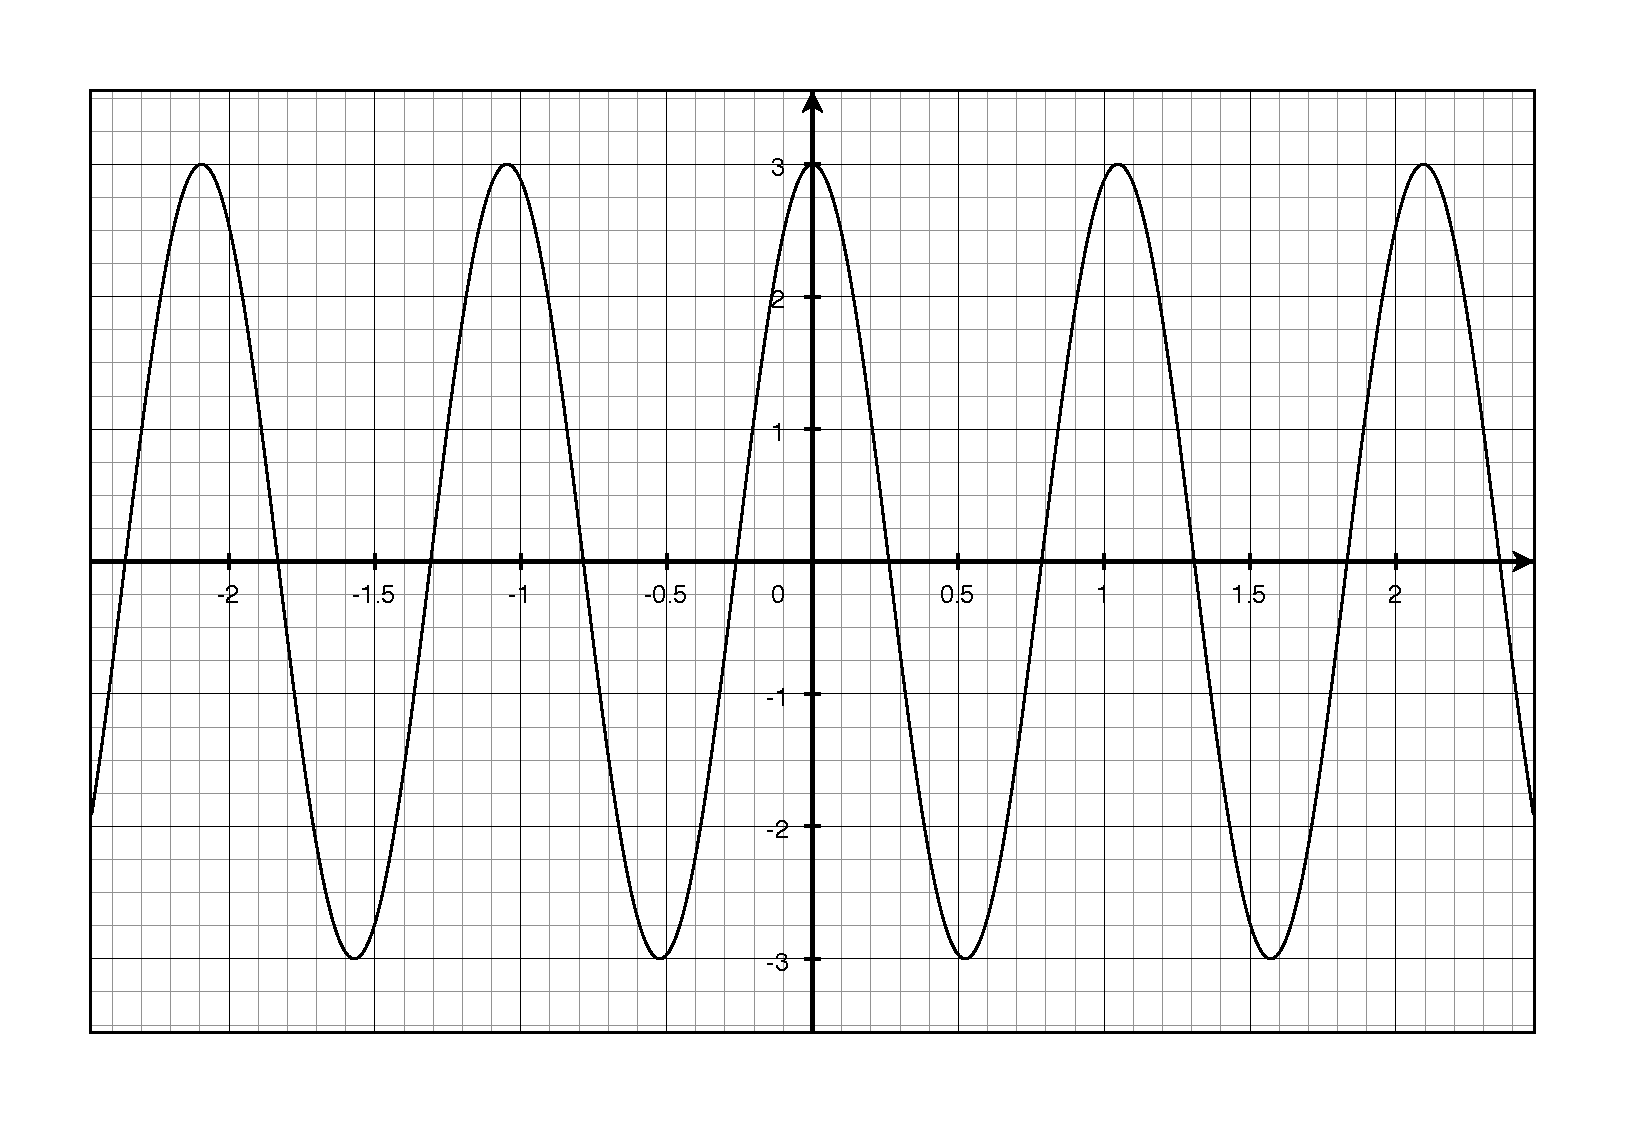
\includegraphics[scale=.3]{question52.eps}
  \caption*{Question 52}
\end{figure}

\item[61]
This looks like a cosine graph with an amplitude of 2 and period of  $2 \pi$ shifted up by 1

\[
  f(x) = 1 + 2 \cos x
\]

\item[62]
This looks like a cosine graph with an amplitude of 2 and period of  $2 \pi$ shifted down by 1

\[
  f(x) = -1 + 2 \cos x
\]

\item[65] $a = -3$, $b = 2$, $c = 0$ or $a = 3$, $b = 2$, $c = \pi$

\item[66] $a=2$, $b = \dfrac{1}{2}$, $c = 0$

\item[73]
\begin{description}
\item[a] 
\[
  t = \dfrac{2 \pi}{\pi / 3} = 6 \text{ seconds}
\]

\item[b]
With 6 seconds per breath, there would be 10 breaths per minute.


\item[c]
\begin{figure}[H]
  \centering
  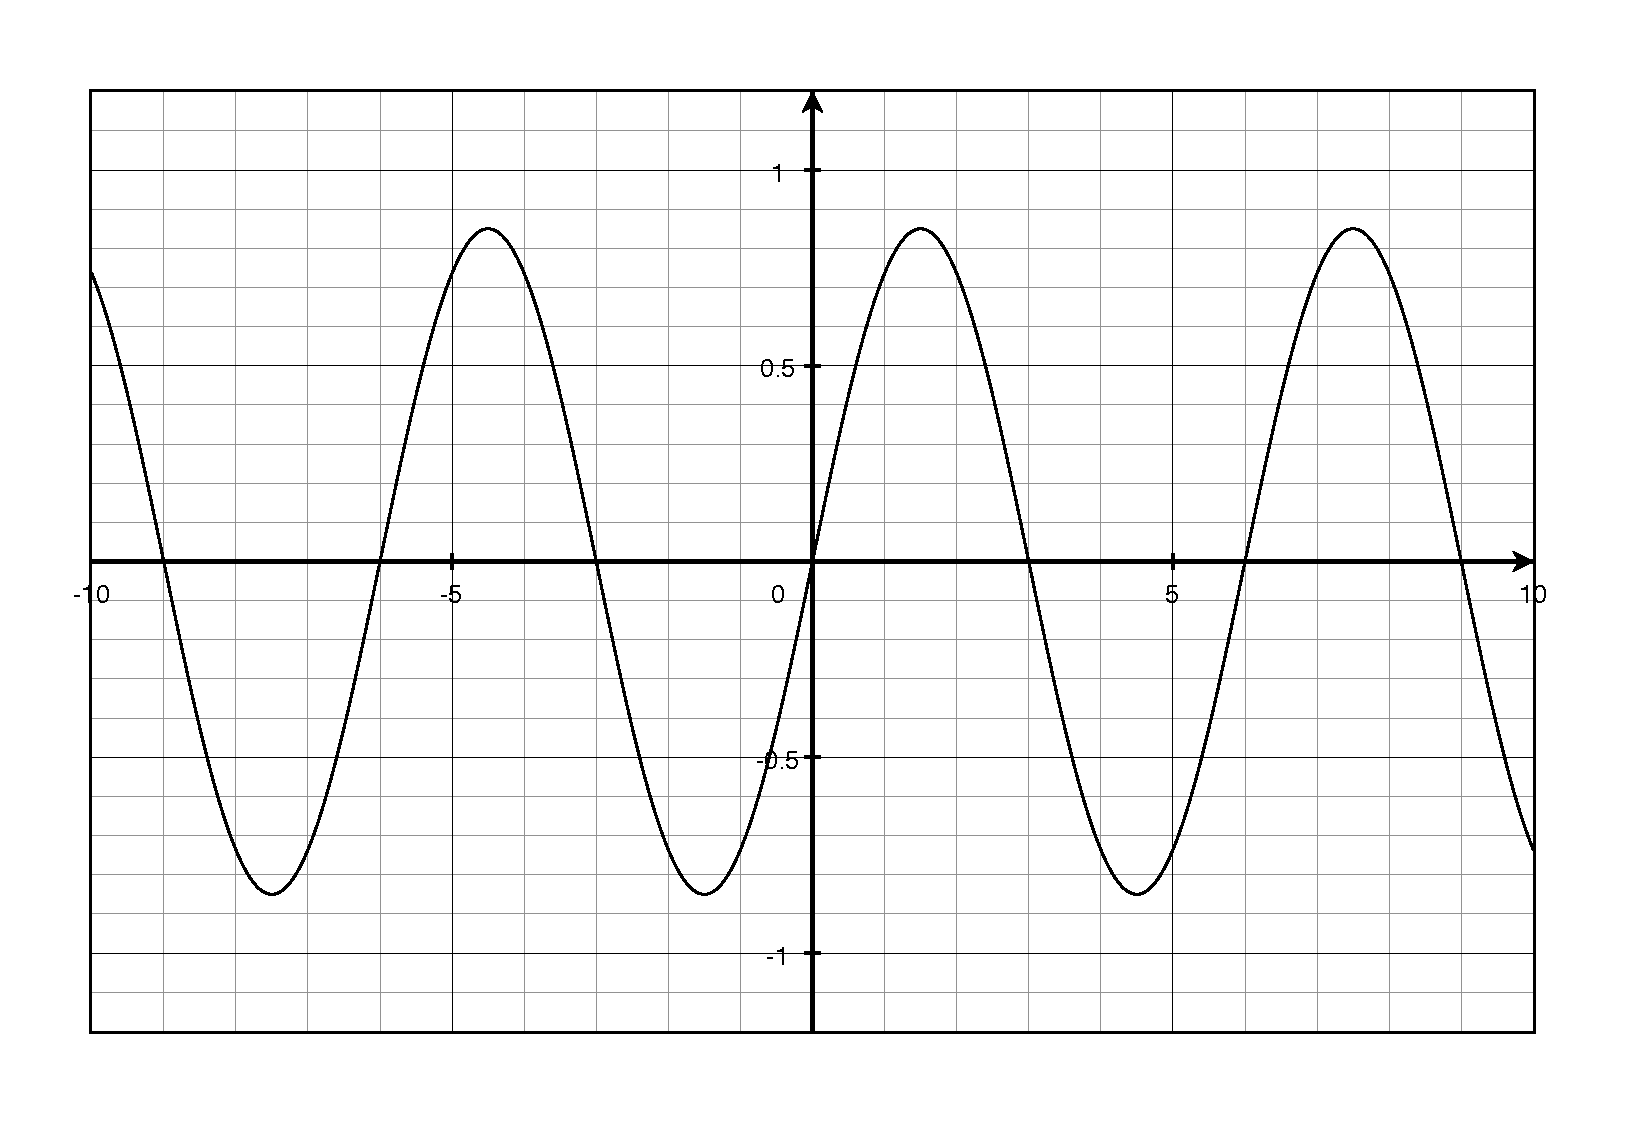
\includegraphics[scale=.3]{question73.eps}
  \caption*{Question 73}
\end{figure}

\end{description}

\item[76]

\begin{description}
\item[a]
\[
  \frac{2 \pi}{5 \pi/3} = \frac{6}{5} \text{ seconds}
\]

\item[b]

\[
  \frac{5 \text{ beats}}{6 \text{ seconds}} \cdot \frac{60 \text{ seconds}}{1 \text{ minute}} = 50 \text{ beats per minute}
\]

\end{description}

\section{Pages 408-409}

\item[1] e
\item[2] c
\item[3] a
\item[4] f
\item[5] d
\item[6] b

\item[7]
\begin{figure}[H]
  \centering
  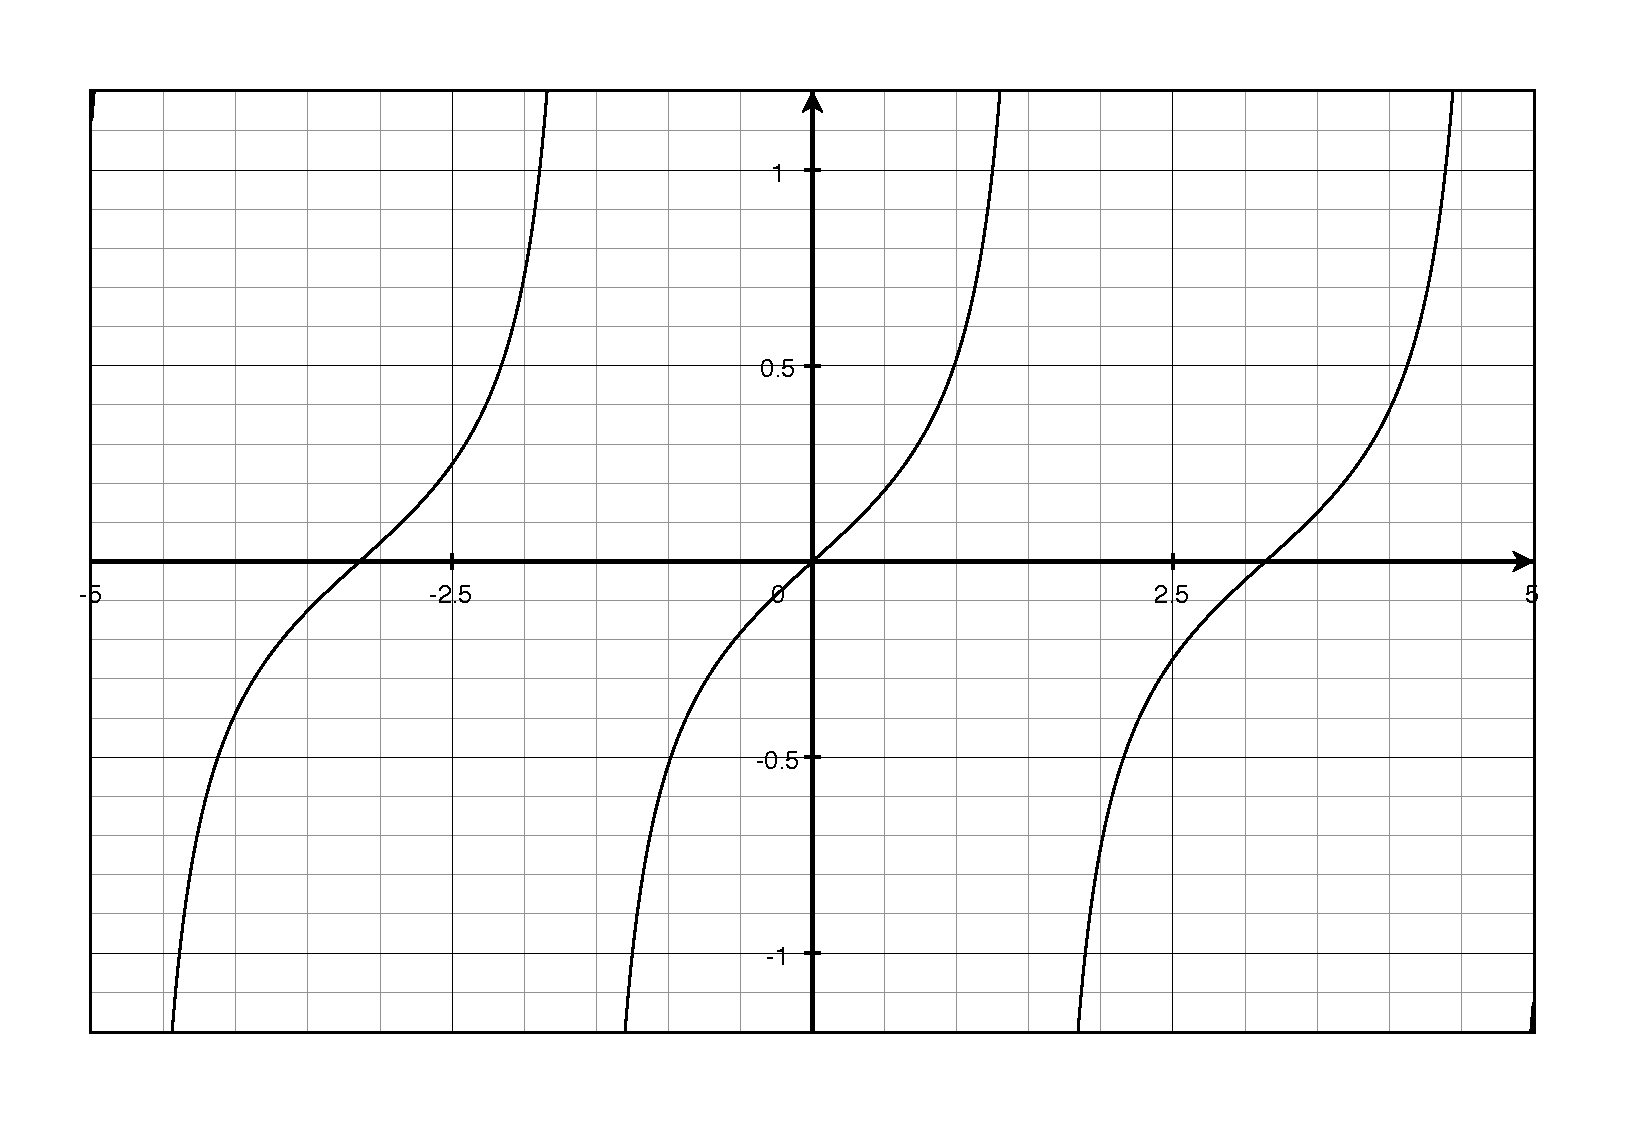
\includegraphics[scale=.3]{question_4.6_7.eps}
  \caption*{Question 7}
\end{figure}

\item[9]
\begin{figure}[H]
  \centering
  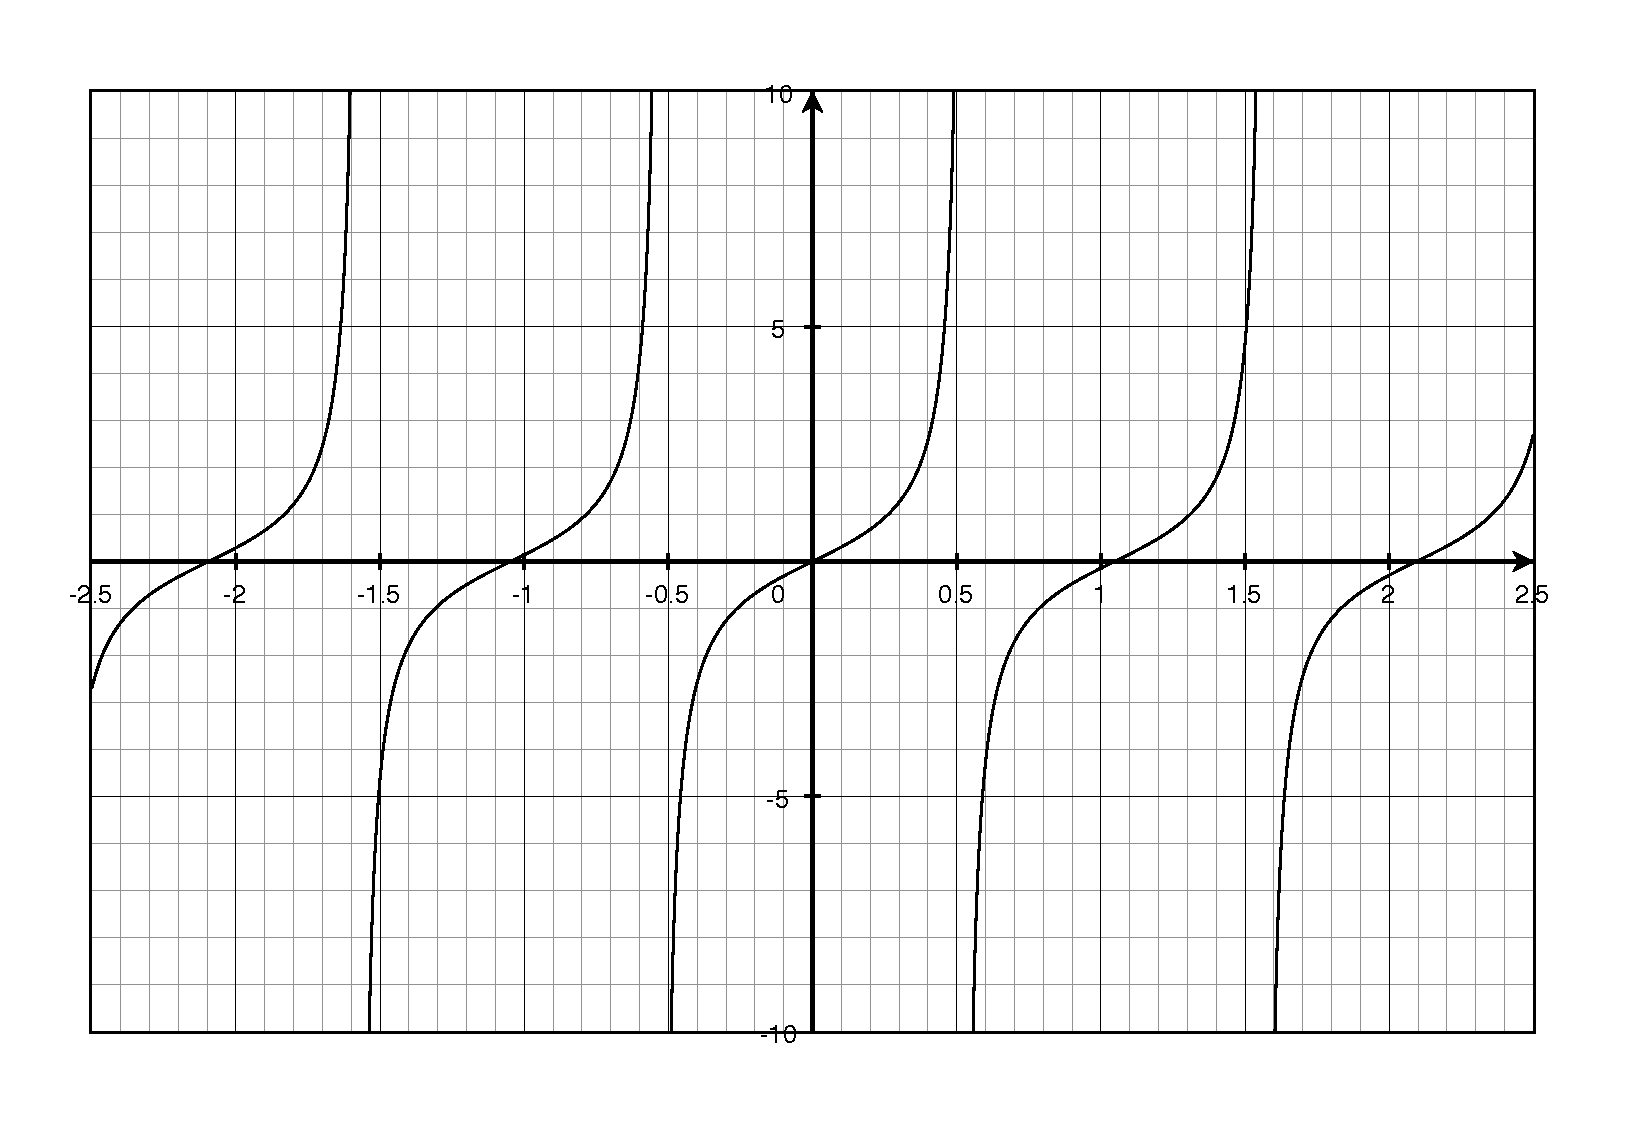
\includegraphics[scale=.3]{question_4.6_9.eps}
  \caption*{Question 9}
\end{figure}

\item[12]
\begin{figure}[H]
  \centering
  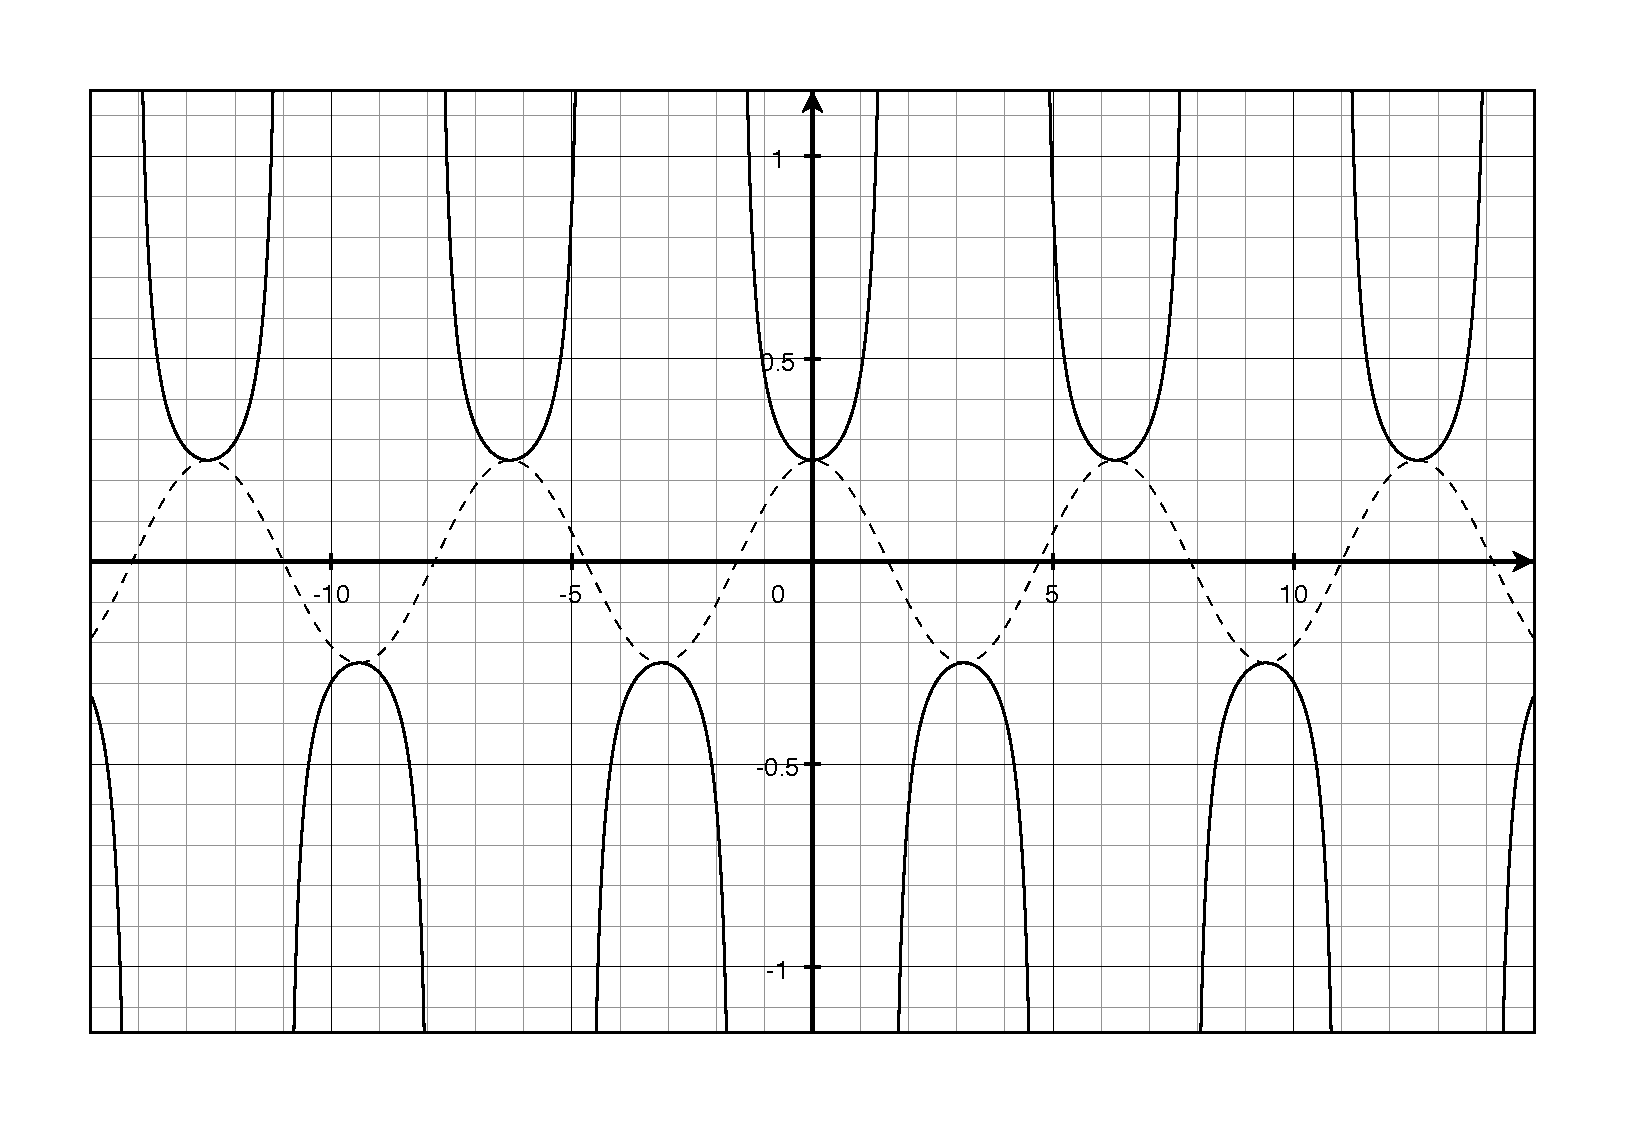
\includegraphics[scale=.3]{question_4.6_12.eps}
  \caption*{Question 12}
\end{figure}

\item[13]
\begin{figure}[H]
  \centering
  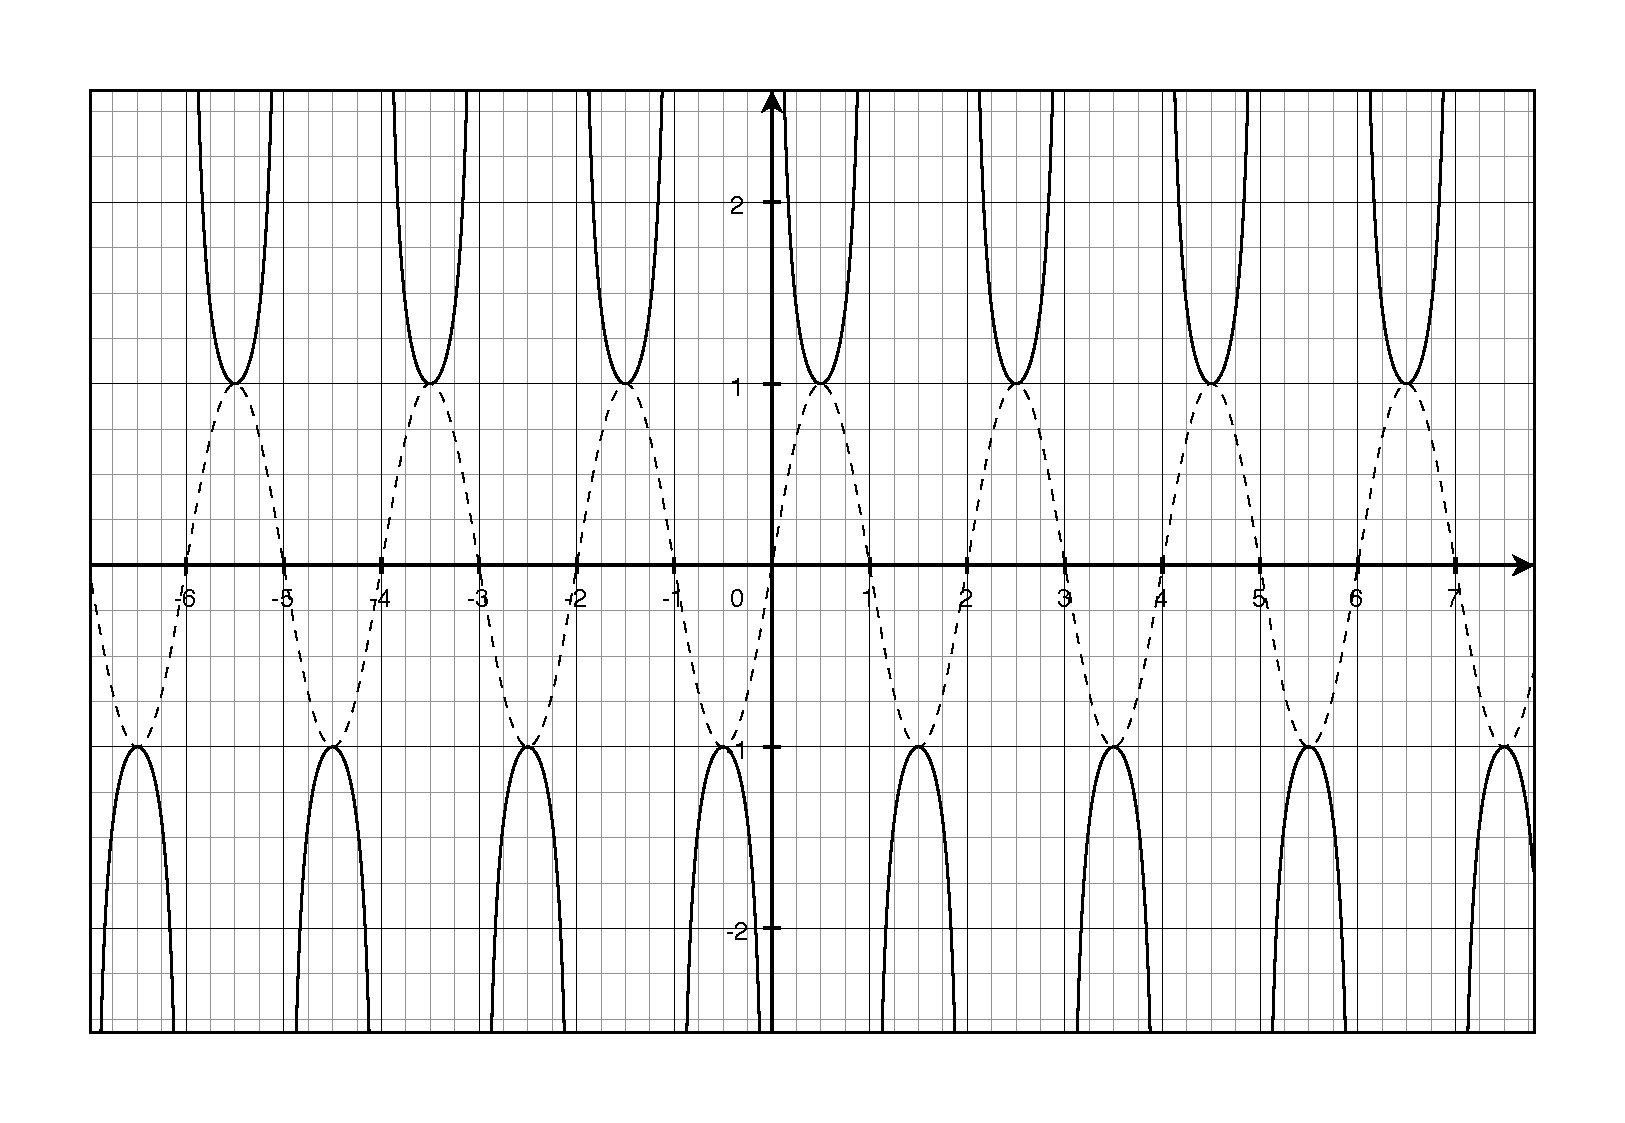
\includegraphics[scale=.3]{question_4.6_13.eps}
  \caption*{Question 13}
\end{figure}

\item[17]
\begin{figure}[H]
  \centering
  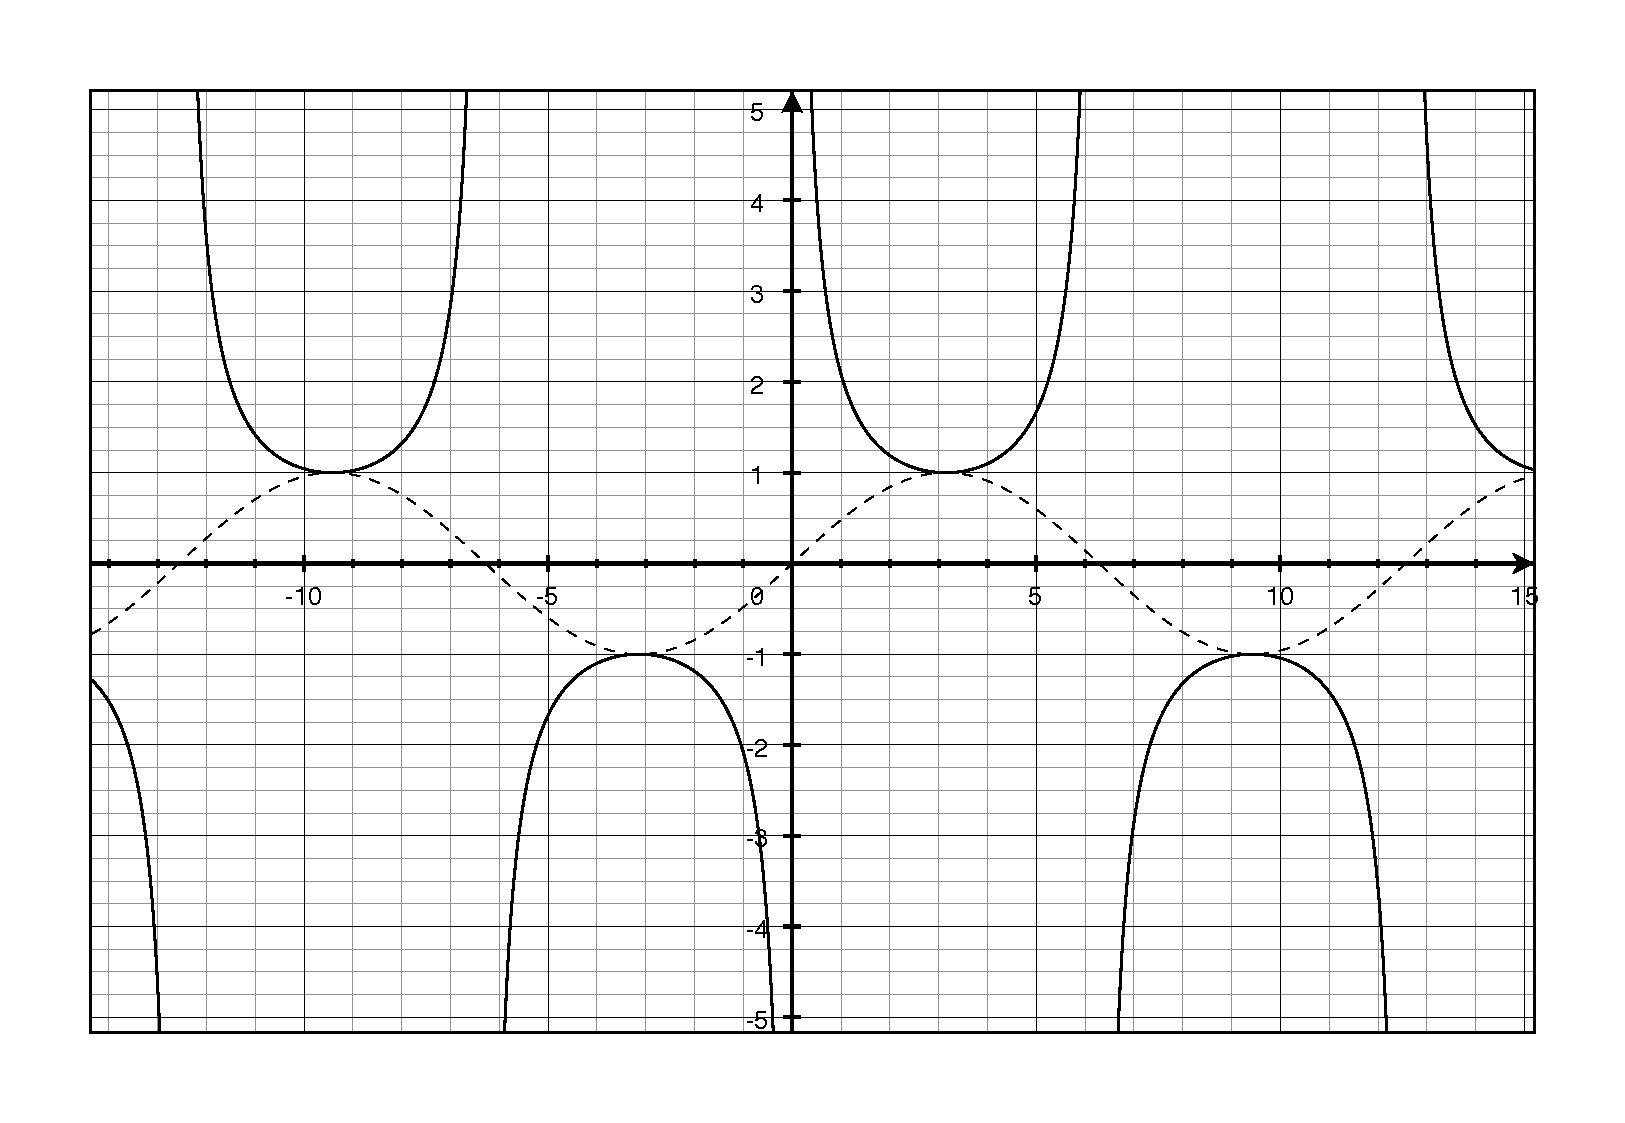
\includegraphics[scale=.3]{question_4.6_17.eps}
  \caption*{Question 17}
\end{figure}

\item[25]
\begin{figure}[H]
  \centering
  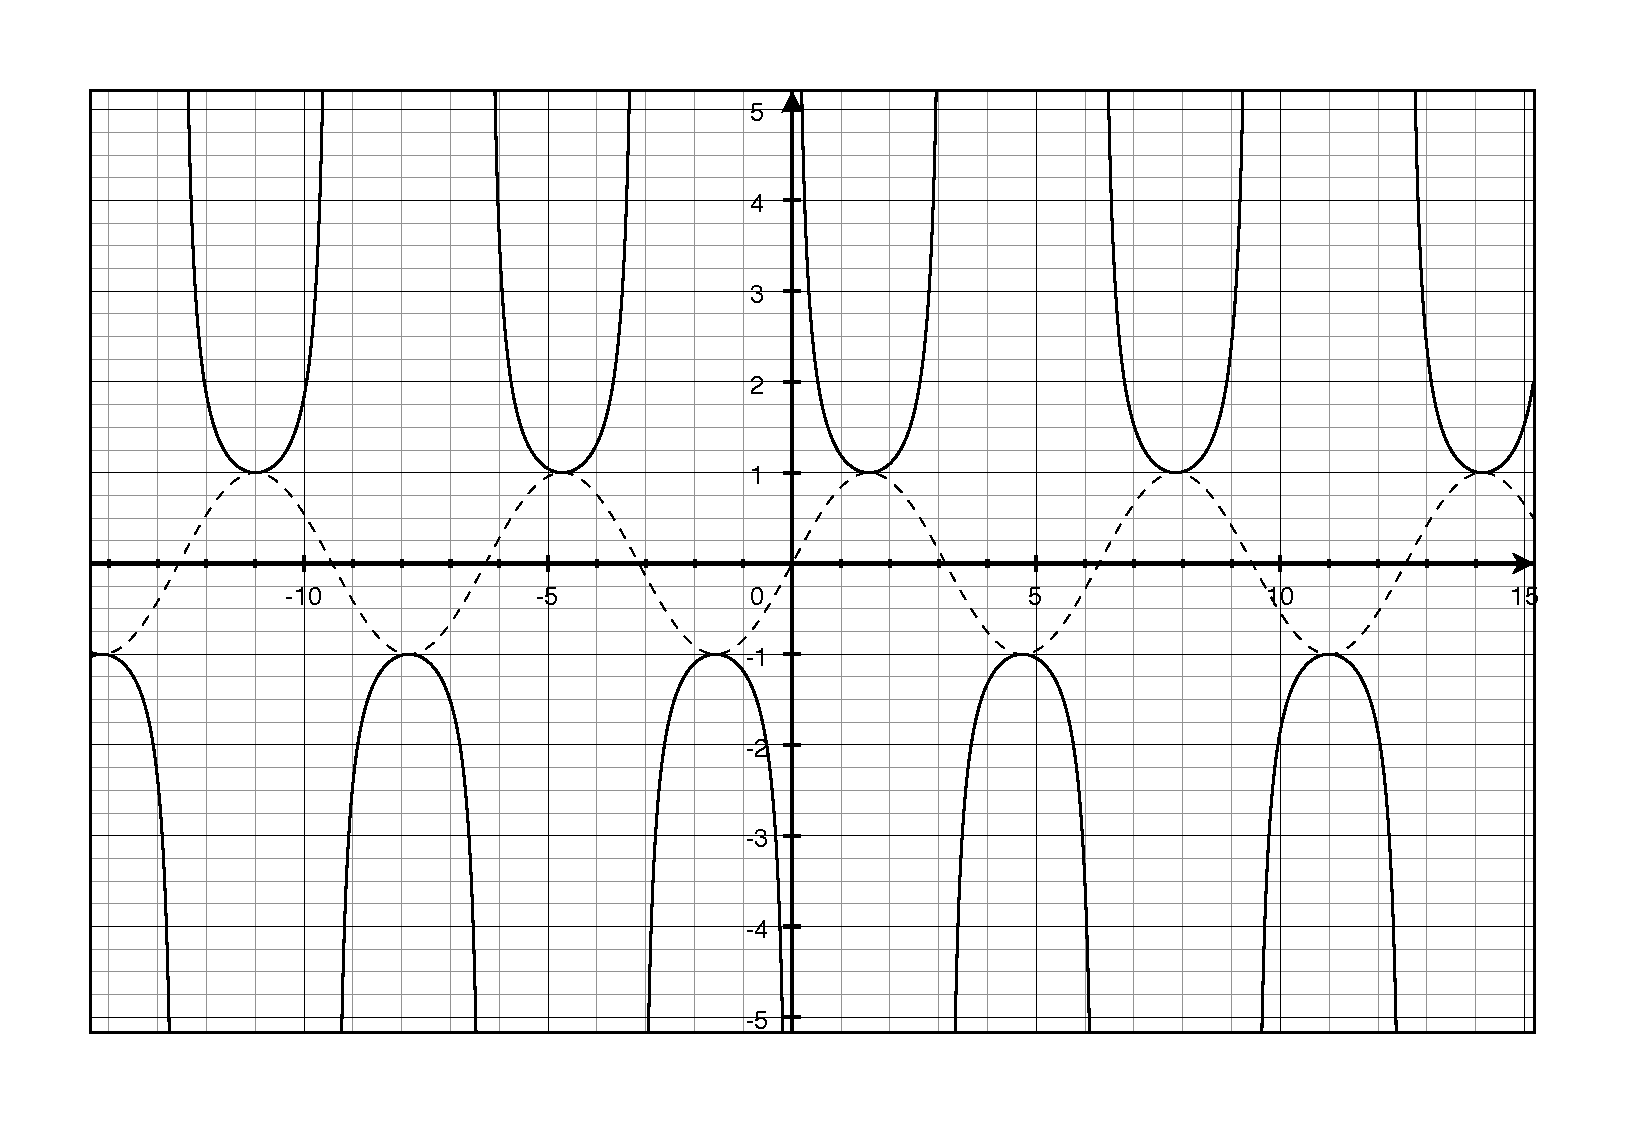
\includegraphics[scale=.3]{question_4.6_25.eps}
  \caption*{Question 25}
\end{figure}

\item[26]
\begin{figure}[H]
  \centering
  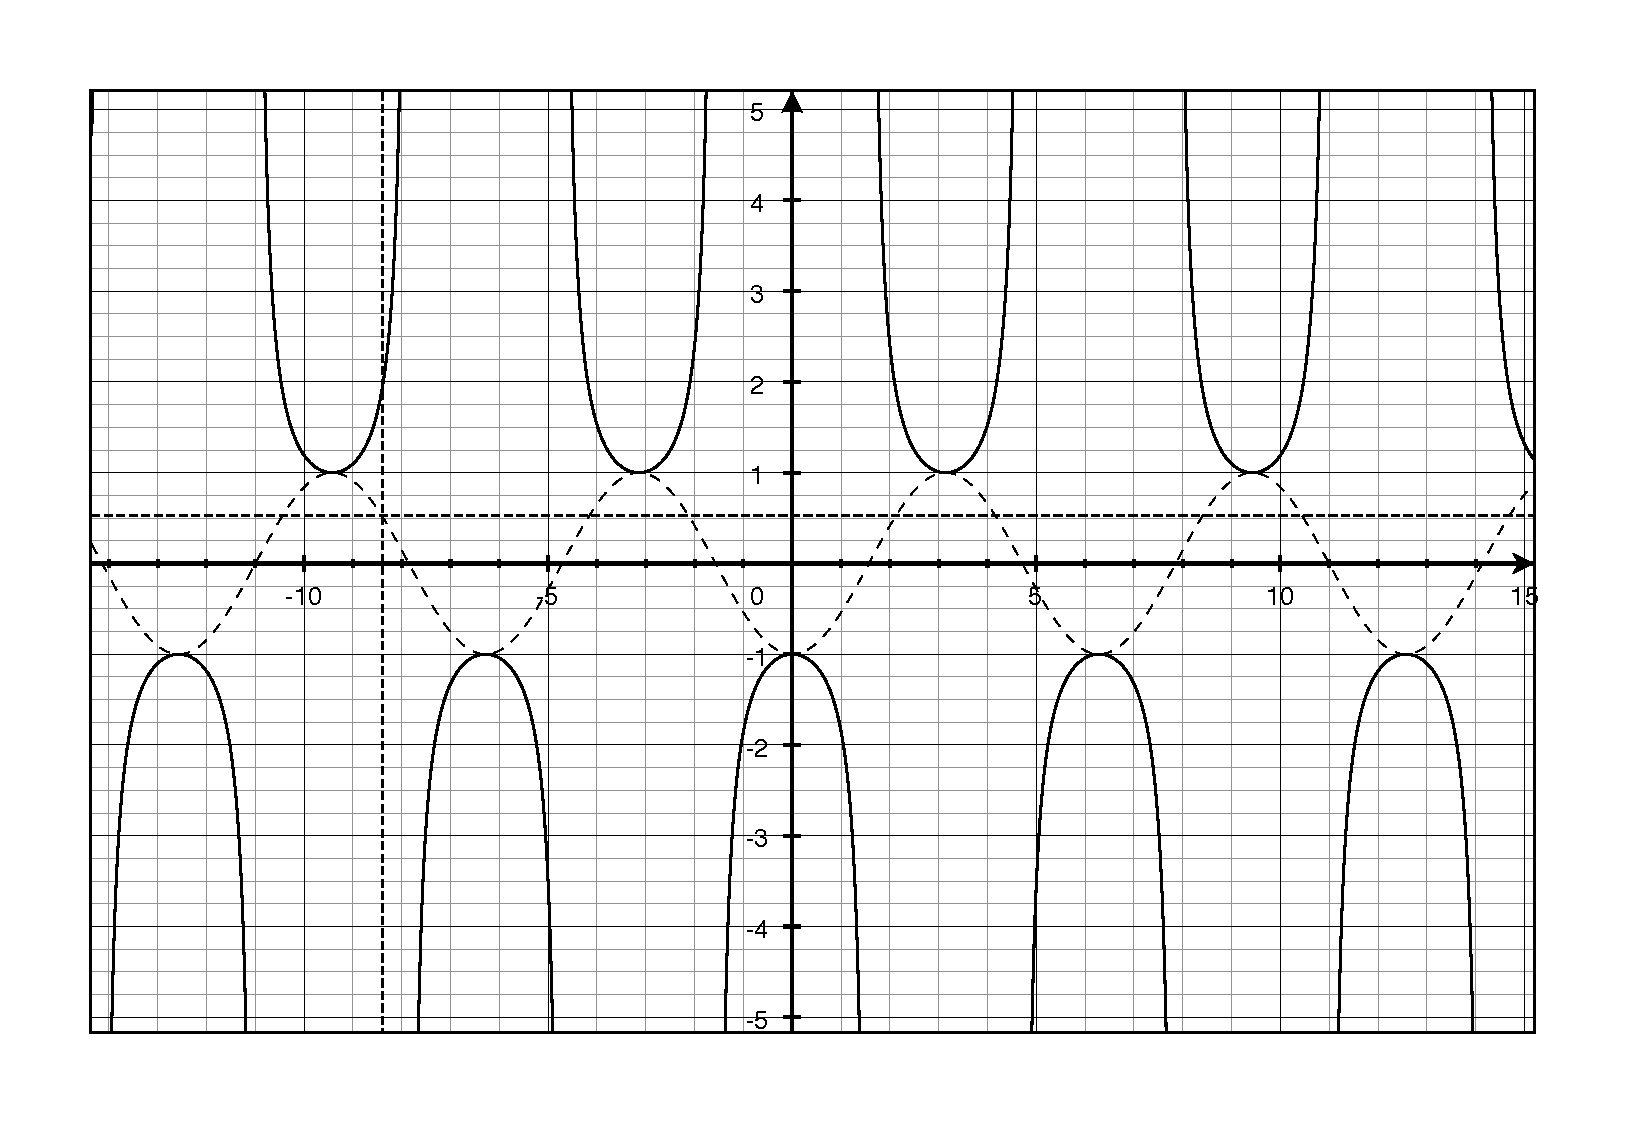
\includegraphics[scale=.3]{question_4.6_26.eps}
  \caption*{Question 26}
\end{figure}

\item[27]
\begin{figure}[H]
  \centering
  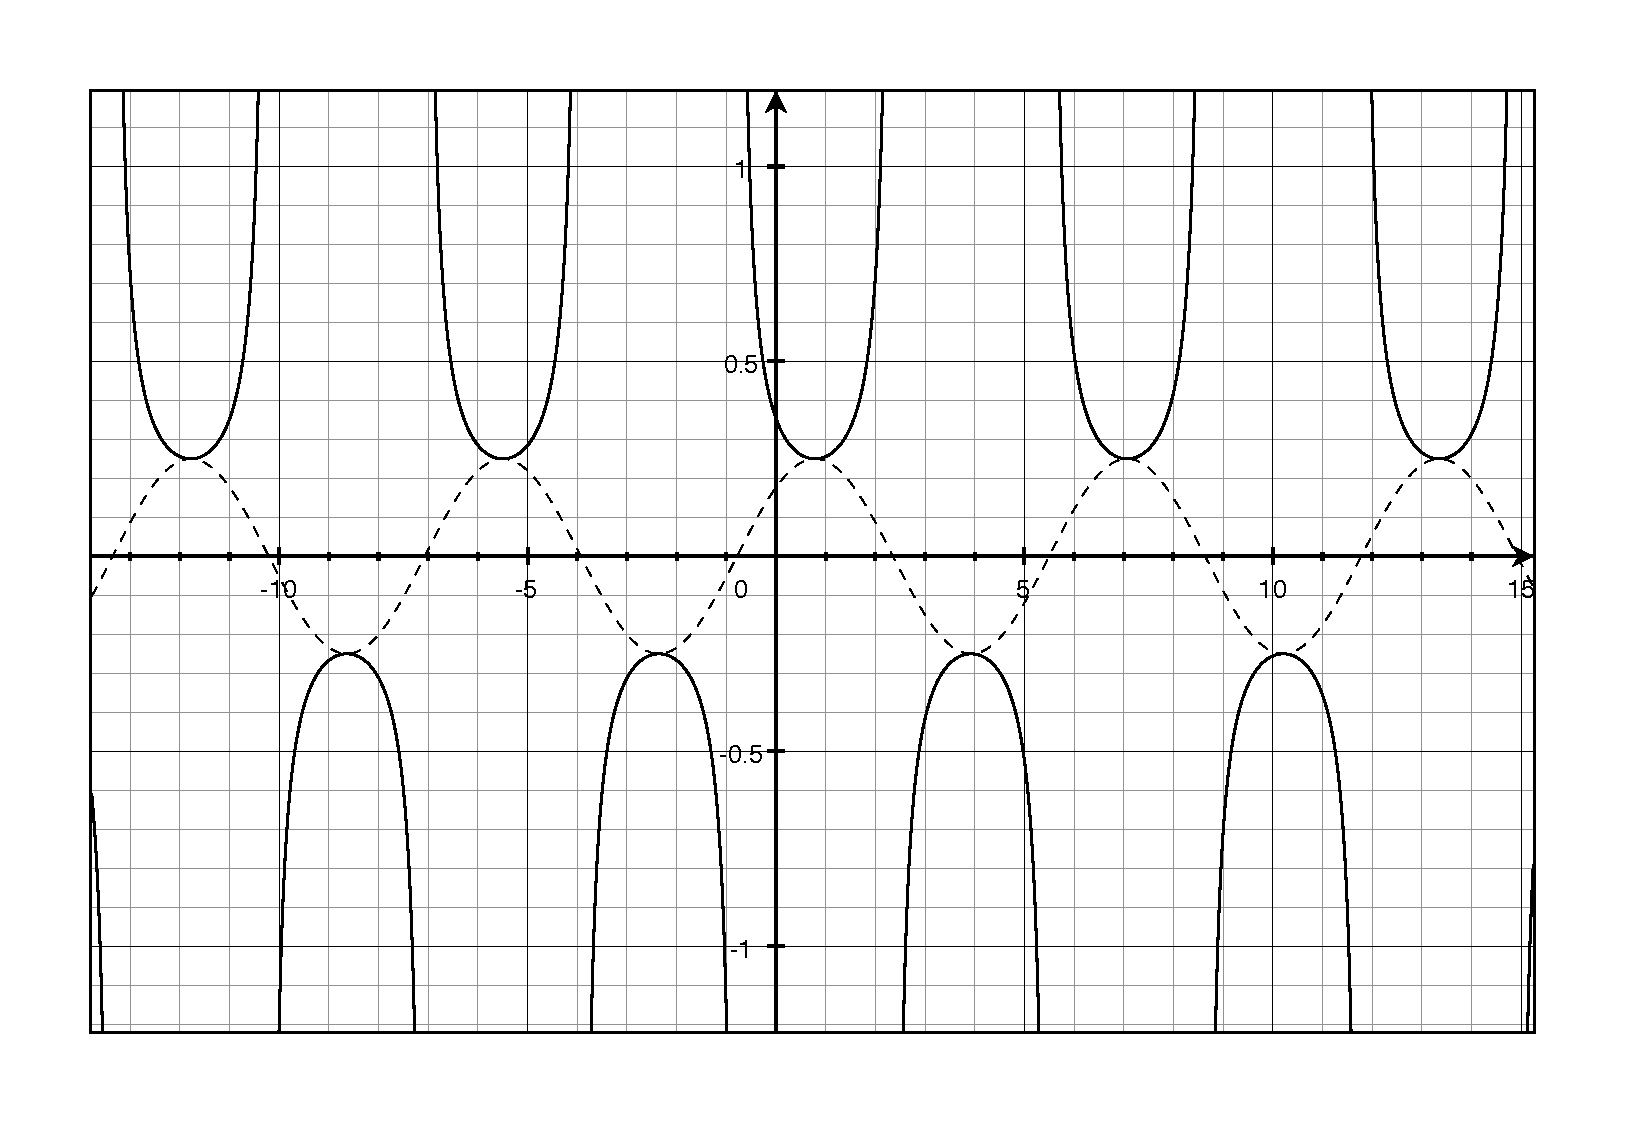
\includegraphics[scale=.3]{question_4.6_27.eps}
  \caption*{Question 27}
\end{figure}

\item[28]
\begin{figure}[H]
  \centering
  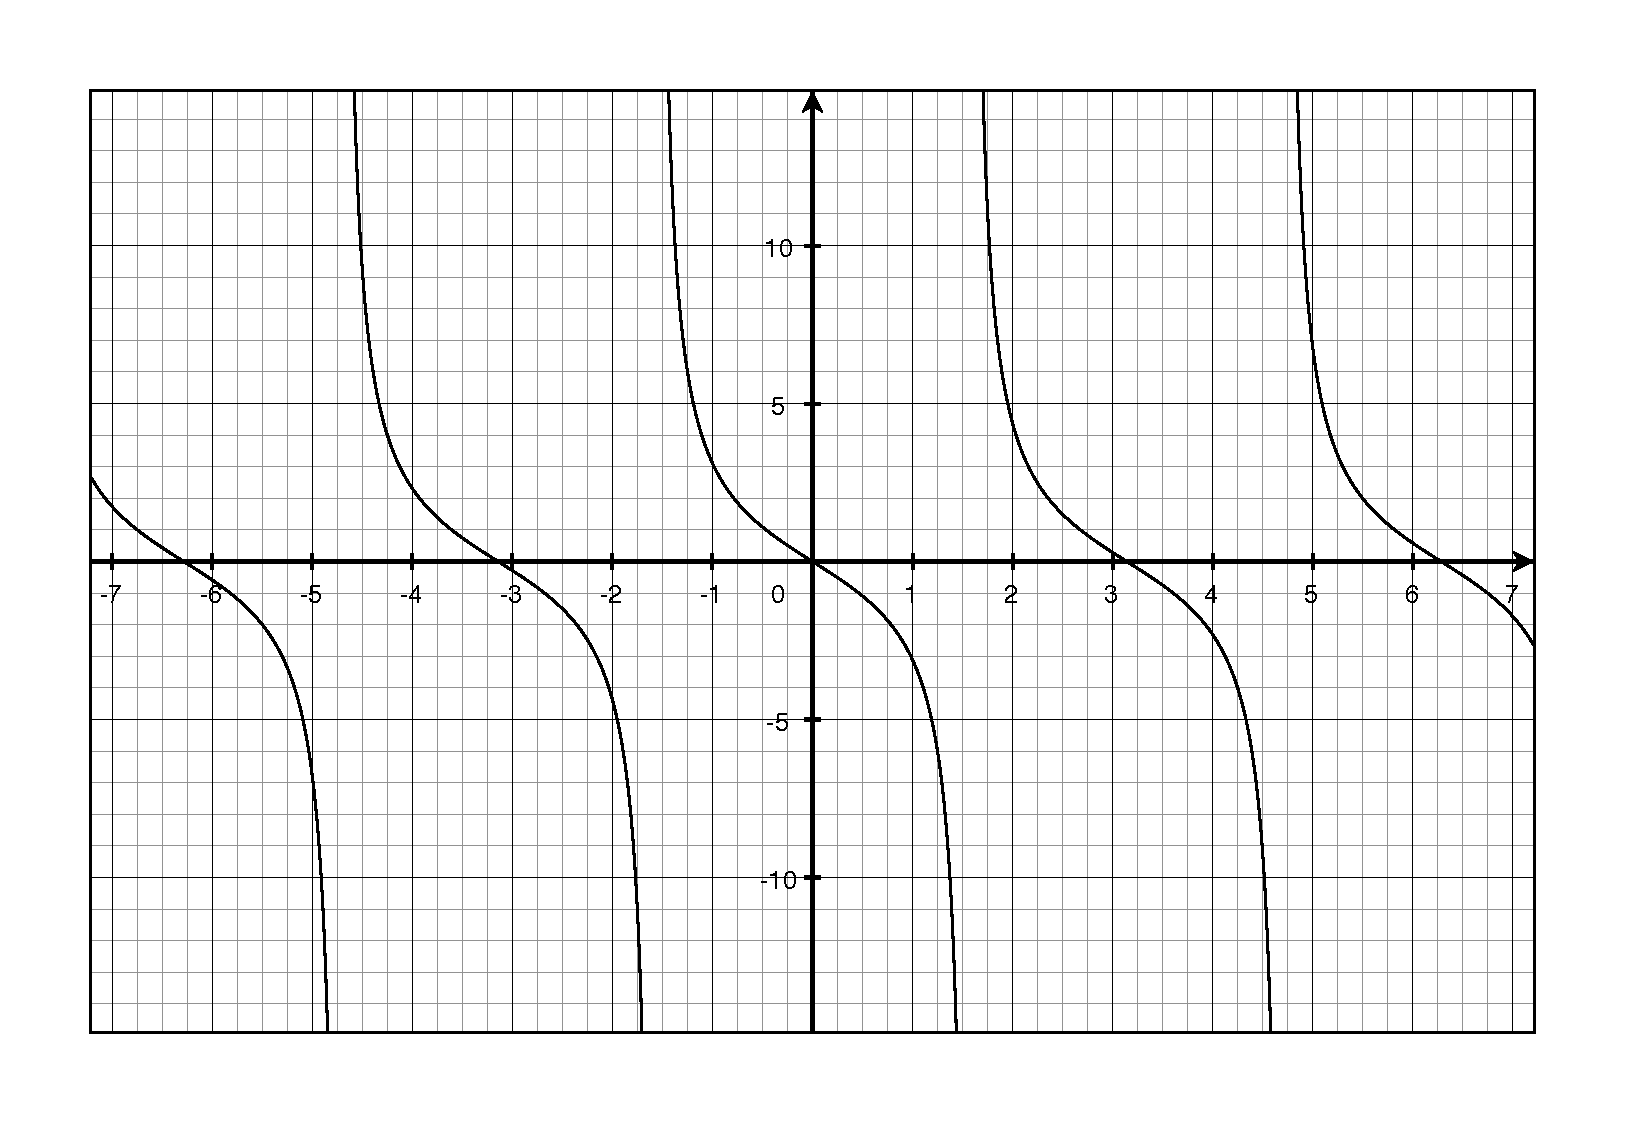
\includegraphics[scale=.3]{question_4.6_28.eps}
  \caption*{Question 28}
\end{figure}

\item[73]

\begin{align*}
  \tan x &= \frac{7}{d} \\
  d &= \frac{7}{tan x} \\
  d &= 7 \cot x \\
\end{align*}

\begin{figure}[H]
  \centering
  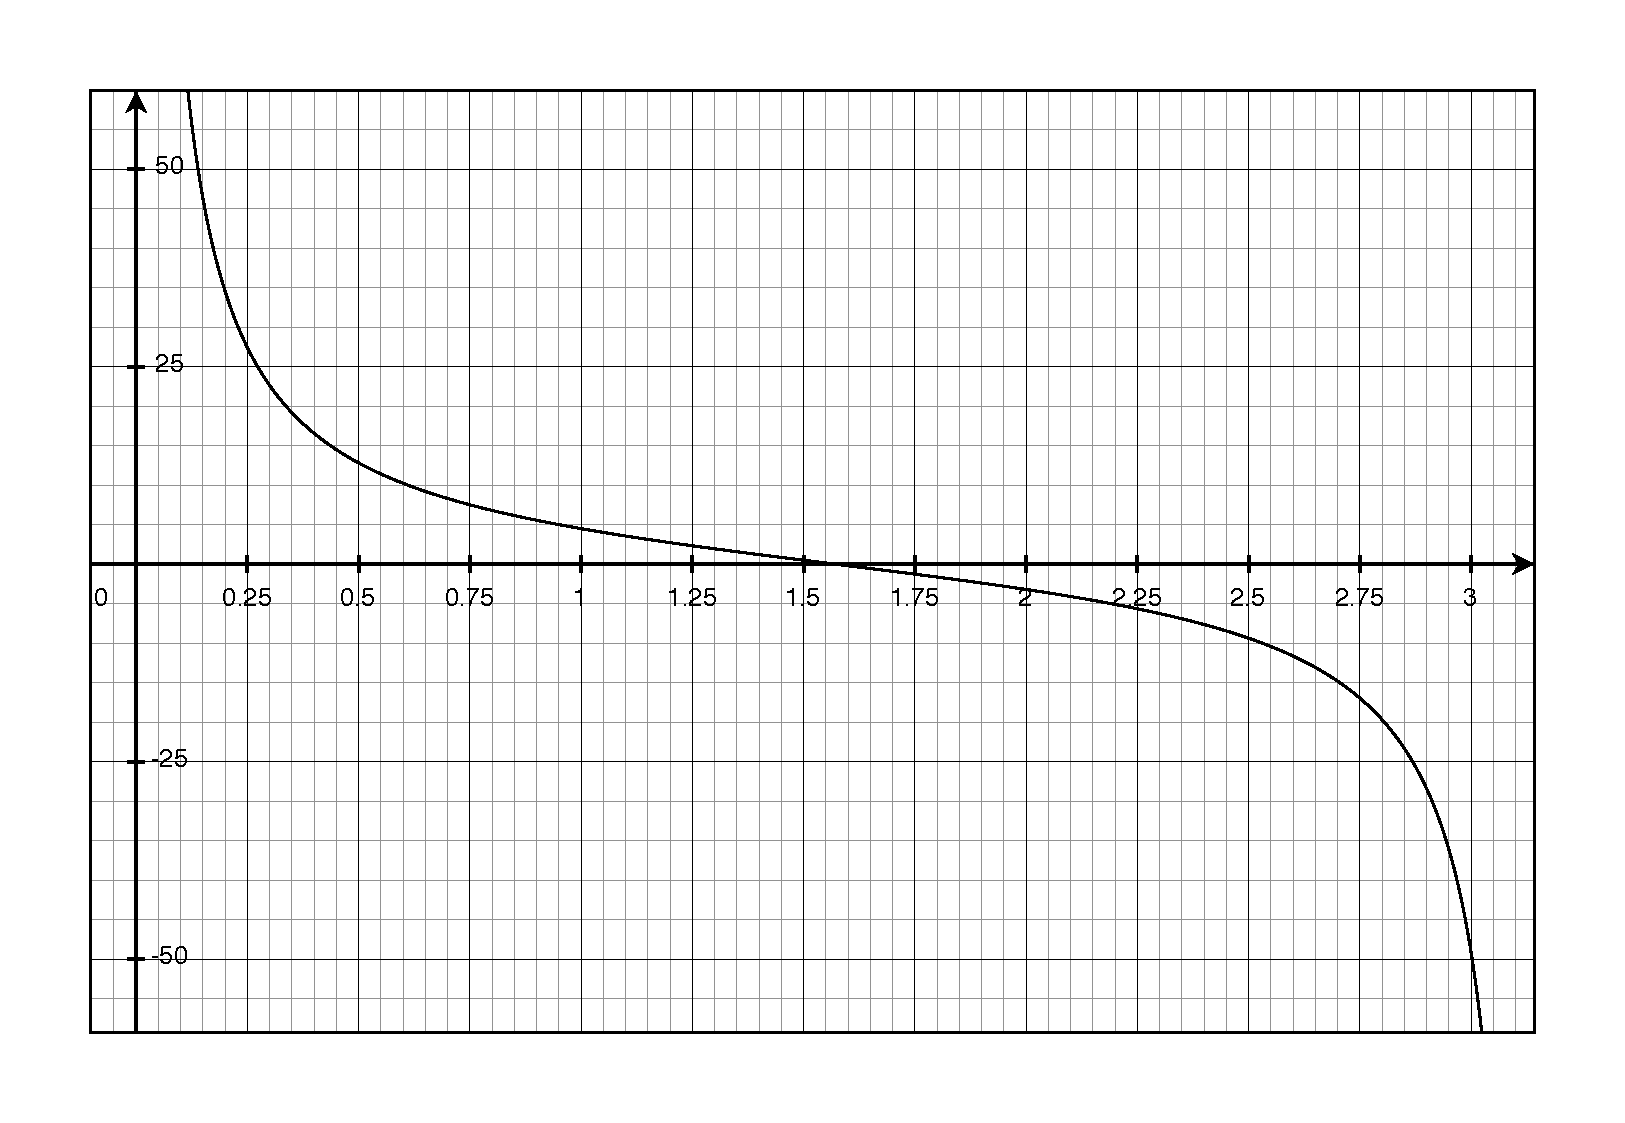
\includegraphics[scale=.3]{question_4.6_73.eps}
  \caption*{Question 73}
\end{figure}

\item[75]

The actual graph is the sum of the two dashed lines.  The sine part of the graph shows the seasonal variation and the
linear part is the company's growth over time.

\begin{figure}[H]
  \centering
  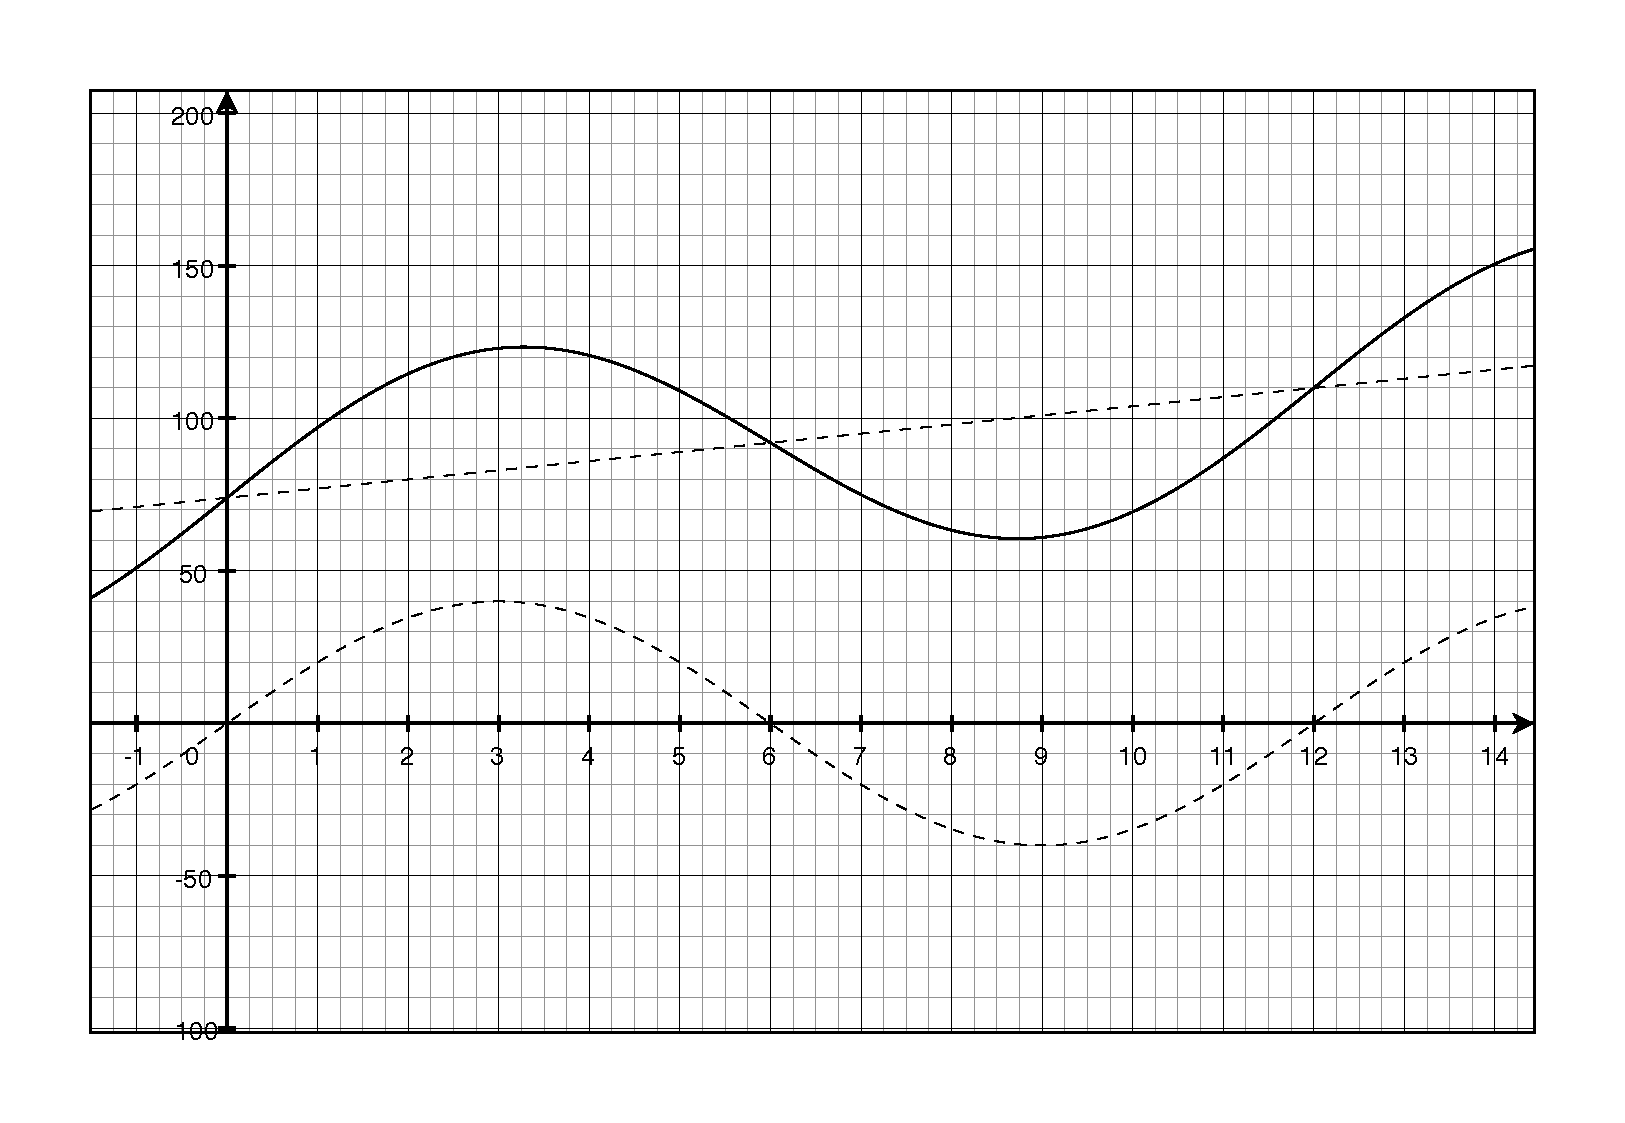
\includegraphics[scale=.3]{question_4.6_75.eps}
  \caption*{Question 75}
\end{figure}

\item[76]

At time zero, there are a lot of prey animals and not many preditors.  So the preditors thrive and eat all the prey
until at time about 5 there are a lot of preditors but the prey is declining.  Since there's not much to eat, the
preditors start declining.  At time 20, the prey is increasing again and the preditors are at a minimum.

The pattern repeats, so the preditor graph always follows the prey graph a little later in time.

\end{description}
\else

\vspace{1 in}

\begin{em}
  All over the place, from the popular culture to the propaganda system, there is constant pressure to make people feel
  that they are helpless, that the only role they can have is to ratify decisions and to consume.
\end{em}

\vspace{.2 cm}
\hspace{1.5 cm} --Noam Chomsky

\fi

\end{document}

